\graphicspath{{design/fig/}}

\chapter{Design}
\section{Design Philosophy}
The aim of this project is to design a impedance spectroscopy system that can be used in a point-of-care setting. Tim Brown's design thinking principles\cite{brownDesignThinking2008} are thus well suited and were used as the bases for the design process. Brown’s approach is characterised by five stages: empathising with the end user, defining a clear problem statement, ideating a wide range of creative ideas, building a quick prototype, and finally testing. These phases are cyclical and allow rapid iteration and learning. This project represents the culmination of this design process, although further iterations of the design process could allow further refinement of the end product.

\subsection{Understanding the end user}
\Ac{POC} diagnostic devices are essential for decentralized healthcare, particularly in resource-limited settings such as rural clinics and community health facilities. While EIS has proven to be a powerful technique for biosensing applications, existing solutions \needscite{present significant barriers to widespread adoption in POC environments.}

Commercial impedance analysers such as the PalmSens4 offer exceptional technical capabilities, including frequency ranges from \SI{10}{\micro\hertz} to 1 MHz, high resolution (18-bit), and data analysis features such as circuit modelling \cite{PalmSens4}. However, these instruments have two critical limitations for \ac{POC} applications. Firstly, they require substantial technical expertise to interpret EIS data, as users must understand the underlying electrochemical principles to extract meaningful diagnostic information. Secondly, commercial systems like the PalmSens4 are prohibitively expensive, with prices \needscite{~\texteuro 15,000}, making them impractical for widespread deployment in clinics, rural health centres, or low-resource settings.

Previous academic projects have successfully demonstrated low cost impedance spectroscopy devices \cite{ebrahimDevelopmentBiosensorEarly2023}\cite{al-aliDesignPortableLowCost2017}\cite{buscagliaSimpleZLowCostPortable2023}, but similarly require users to manually analyse impedance spectra and possess an understanding of EIS principles to interpret the results. This technical barrier prevents POC personnel from using these devices effectively.

\Ac{POC} healthcare providers require a device that performs impedance-based biosensing but abstracts the complexity away from the user, presenting results in an intuitive way. Quantitative results, rather than qualitative results are sufficient to indicate the need for referral to a specialist and further testing. 

\subsection{Problem Statement}

\textbf{How can we design a low-cost, easy-to-use impedance analyzer for biosensing applications that eliminates the need for specialized knowledge, enabling point-of-care personnel to test for multiple biomarkers?}
\newline
This problem statement encapsulates three critical design requirements :
\begin{enumerate}
    \item Accessibility: \needscite{The device must process raw impedance measurements and convert them to meaningful outputs, removing the need for users to understand Nyquist plots, equivalent circuit models, or phase angle analysis. Running from a battery and being able to operate without a computer are also necessities in rural settings.}
    \item Affordability: \rephrase{The total system cost must remain under R4,500 (approximately €220), making it orders of magnitude more affordable than commercial alternatives like the PalmSens4 at €15,000, thereby enabling widespread deployment in resource-limited settings}.
    \item Multiplexing capability: In resource constrained \ac{POC} environments, healthcare professionals often face high patient loads. Due to this, multiplexed \ac{POC} testing is of increasing importance for clinical screening \cite{dincerMultiplexedPointofCareTesting2017}. This allows the screening of multiple analytes with minimal involvement from healthcare professionals.
\end{enumerate}

\section{Functional Design Overview}
The system can be broken up into multiple subsystems, each fulfilling a specific function in order to create a complete device that meets the requirements. On the most basic level the device consists of the \acp{DUT}, an impedance analyser and a user interface. The DUT is the biosensor that interacts with the analyte and whose impedance characteristics change based on the analyte concentration. A multiplexer is used to interface between multiple DUT's and the impedance analyser. The impedance analyser can be further broken down into the \rephrase{power electronics}, excitation stage, voltage and current measurement stages and finally the processing that uses an STM32. The user interface is based on an ESP32 and communicates with the impedance analyser through UART.

\todo{Breek impedance analyser op in further subsystems}
Discuss wat ons wil bereik en hoe ons dit gan opbreek. Beskryf hoe die circuit die beginsels van biosensors en EIS in ag moet neem, basies wat dit moet doen, hoekom multiplexing en ja dan hoe daai overall doel in gedeeltes opgebreek word.

\begin{figure}[H]
    \centering
    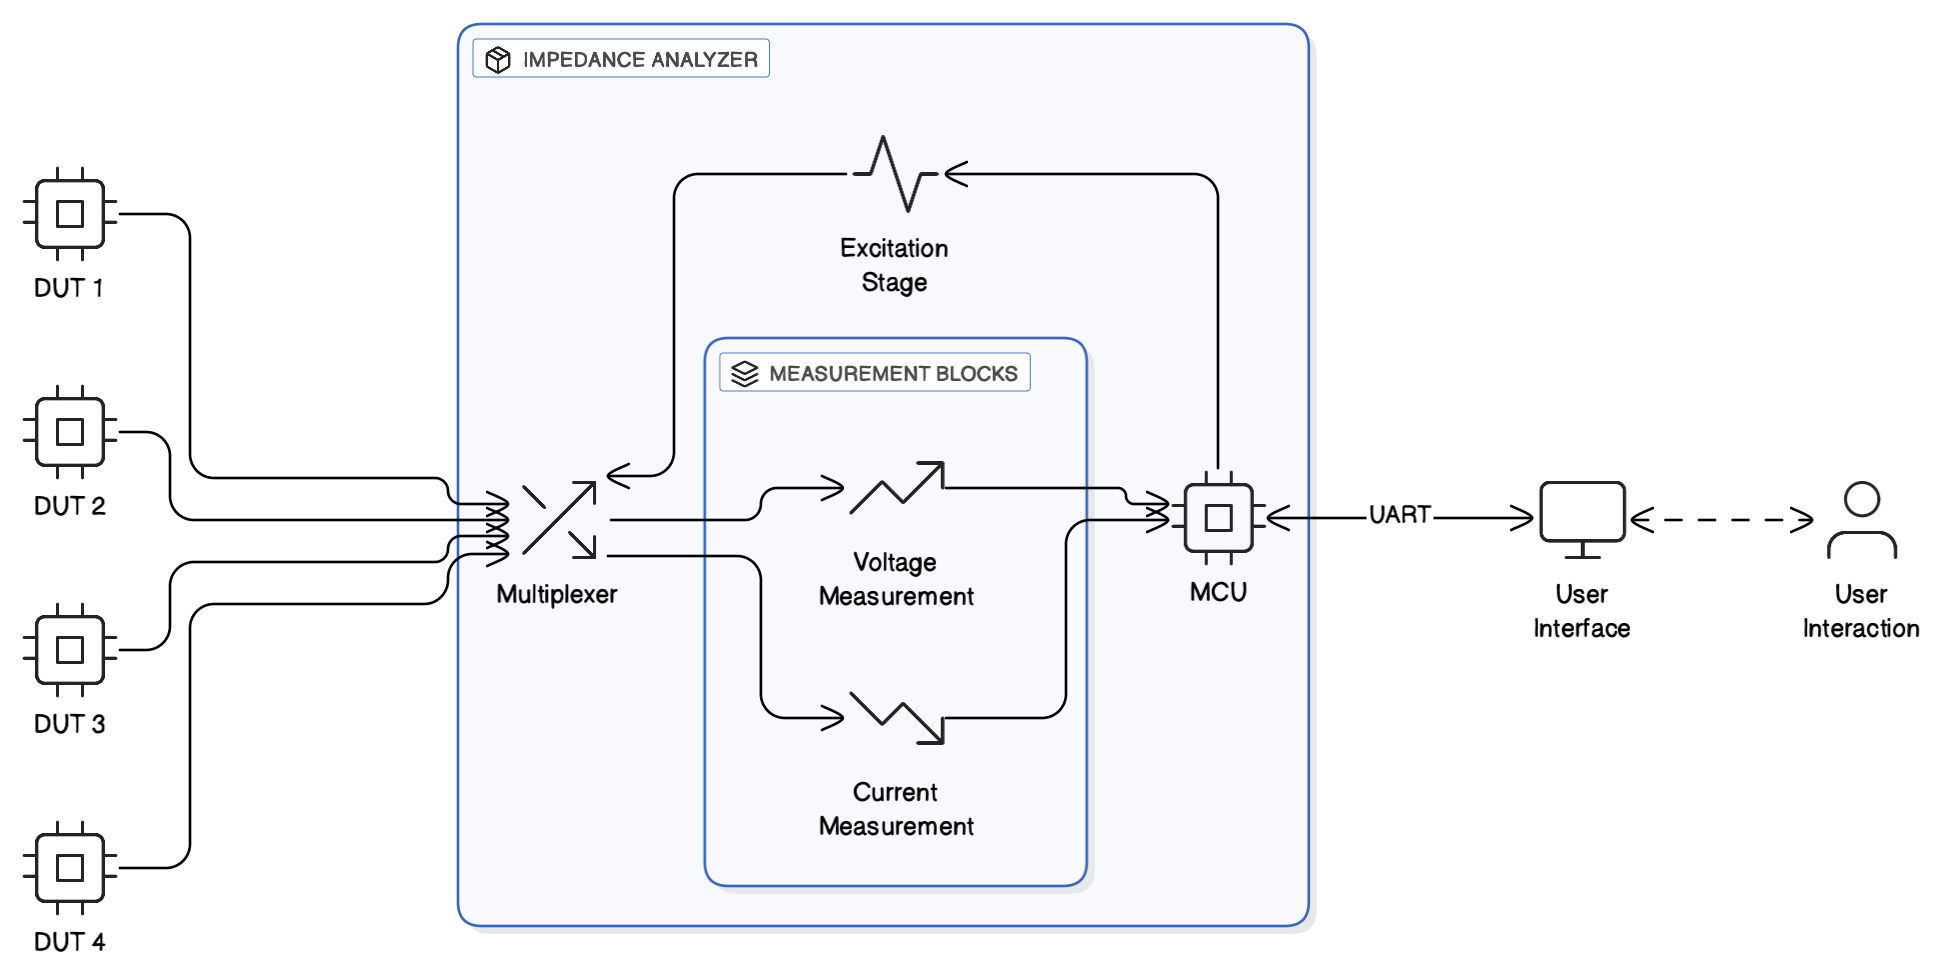
\includegraphics[width=0.8\textwidth]{SystemOverview.png}
    \caption{System Overview}
    \label{fig:system_overview} 
\end{figure}

\section{Analogue Frontend Design}

\subsection{Excitation}\label{subsec:design_excitation}
The easiest way of producing a controlled voltage signal is using a \ac{DAC}. Both dedicated \acp{DAC} and \acp{DAC} built into \acp{MCU} were possible options.

To avoid establishing a DC bias at the electrode–electrolyte interface, the generated excitation must be centred around a stable reference potential. This can be achieved by shifting the \ac{DAC} output to be biased around ground using a level-shifting op-amp circuit. However, this requires providing all analogue circuitry with a negative supply rail. This project instead uses a buffered virtual ground reference at 1.65 V (3.3 V/2) as the midpoint for all analogue circuitry. This approach ensures no DC bias is applied to the \ac{DUT} whilst negating the need for negative supply rails.

The anti-aliasing filter must provide sufficient attenuation at the Nyquist frequency ($f_s/2$) to ensure any aliased content falls below the \ac{DAC}'s noise floor. For the 12-bit \ac{DAC} found in the STM32F303K8, equation \ref{eq:dac_range} gives a dynamic range of 74 dB. 

\begin{equation}
    \text{Dynamic Range} = 6.02n + 1.76 
    \label{eq:dac_range}
\end{equation}

The filter's passband must remain flat at the desired signal bandwidth to avoid distorting the amplitude or phase of the intended output. Due to these requirements, a fixed frequency AA filter is unsuitable when generating frequencies from 1 Hz to 100 kHz. Many variable AA filter ICs exist, but most require changing resistor values to set the cutoff frequency, which is impractical when many frequencies are needed. 

The LTC1069 proved to be the only viable option. It provides an 8th order lowpass filter that approximates a raised cosine response (with $\alpha=1$). It has a cutoff frequency of up to 120 kHz (200 kHz when using $\pm5$ V supply rails) set by an external clock and a linear phase response \cite{LTC10697CS8PBF}. The clock-tunable nature is ideal for this project, allowing easy adjustments through a timer on the STM.

To maximise voltage resolution and minimise noise, the full linear range of the \ac{DAC} is utilised when generating the signal. This requires that the \ac{DAC} output signal is attenuated from 3 Vpp to the desired 10 mVpp using an inverting op-amp. From equation \ref{eq:inv_opamp_gain}, $R_{f}=1 k\Omega$ and $R_{in}=300 k\Omega$ can be calculated as suitable values.

\begin{equation}
    A_v = \frac{V_{out}}{V_{in}} = -\frac{R_f}{R_{in}}
    \label{eq:inv_opamp_gain}
\end{equation}

\begin{figure}[]
    \centering
    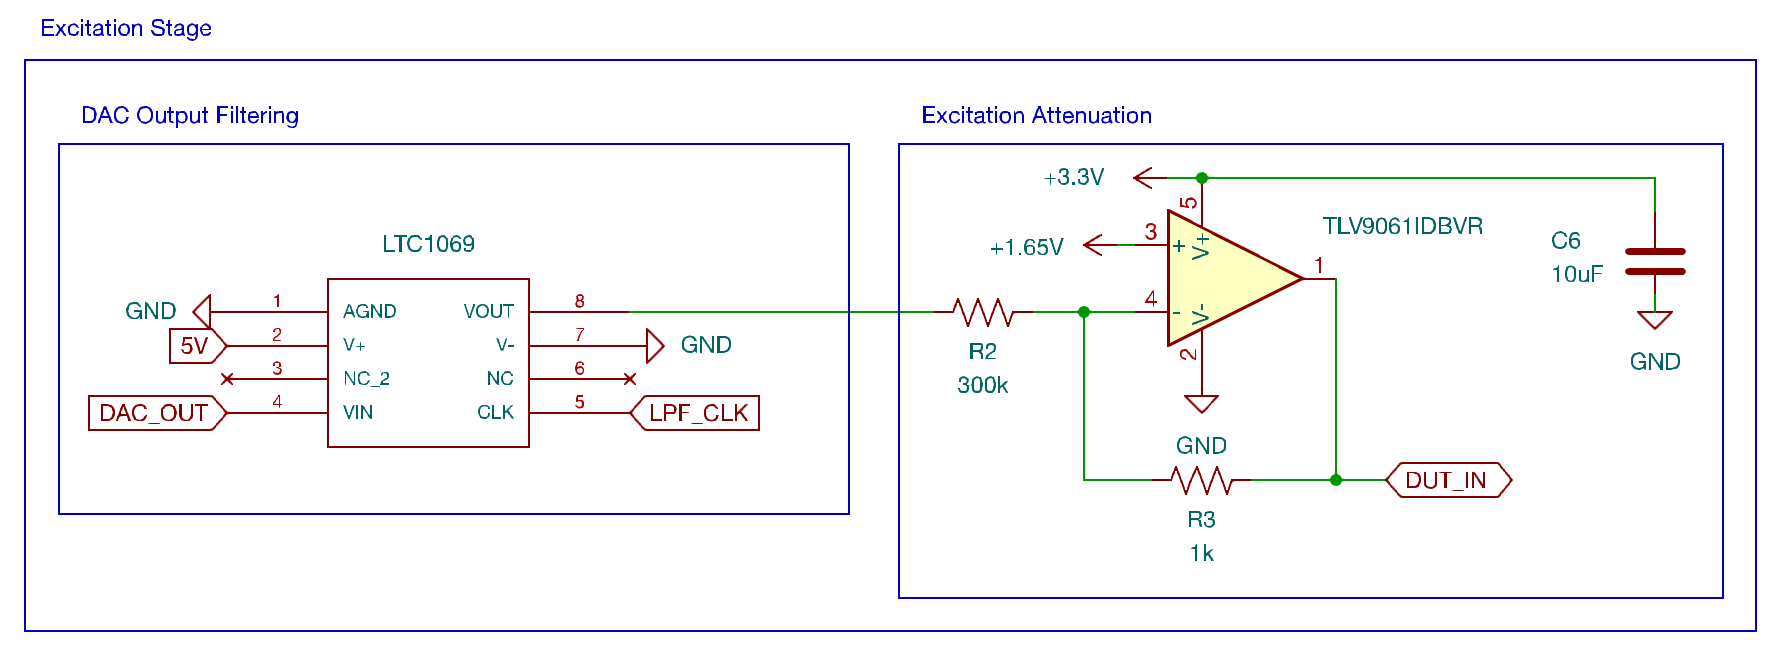
\includegraphics[width=\textwidth]{ExcitationSchem.png}
    \caption{Complete Excitation Stage Circuit}
    \label{fig:excitation_stage_circuit}
\end{figure}

\subsection{Voltage Measurement}
The voltage measurement stage is responsible for accurately measuring the voltage across the \ac{DUT} during excitation. The expected voltage levels across the \ac{DUT} are in the range of 10 mVpp, which is too small to be measured directly by the \ac{ADC} of the STM32F303K8, which has an input range of 0-3.3 V. To fully utilise the \ac{ADC}'s resolution and sensitivity, the voltage signal must be amplified to match the \ac{ADC}'s input range. This requires a gain of approximately 300 V/V (from 10 mVpp to 3 Vpp). However, amplifying the signal by such a large factor in a single stage would introduce significant phase shifts and gain reductions at higher frequencies due to the gain-bandwidth product limitations of op-amps. To mitigate this, a two-stage amplification approach is employed.

The INA331 instrumentation amplifier was selected for the first stage of voltage measurement due to its combination of low offset voltage, high common-mode rejection and low input bias current. The INA331 features a typical offset voltage of 250 µV, which represents the inherent DC error between the input terminals when no differential signal is applied. It directly adds to the measured voltage, creating a systematic DC error that must be considered in calibration. The low input bias current of 0.5 pA avoids loading the \ac{DUT} and influencing current measurements. 

The device provides an internal gain of 5 V/V, configurable to higher gains through external resistors according to the relationship $G = 5 + 5\times \frac{R_2}{R_1}$. Choosing $R_1=1 k\Omega$ and $R_2=2 k\Omega$ results in a gain of 15 V/V. 

\todo{Discuss why bandwidth is important instead of jumping straight into it}
\Ac{GBW} represents the -3 dB bandwidth of an op-amp at unity gain. The -3 dB bandwidth of the op-amp can be calculated for a specific gain using equation \ref{eq:GBW}, where $A_{noise}$ represents the noise gain calculated in equation \ref{eq:noise_gain}. The use of noise gain accounts for non-ideal feedback effects and circuit imperfections \cite{fiore53GainBandwidthProduct2018}.

\begin{equation}
    f_c = \frac{GBW}{A_{noise}}
    \label{eq:GBW}
\end{equation}
\begin{equation}
    A_{noise} = 1 + \frac{R_f}{R_{in}}
    \label{eq:noise_gain}
\end{equation}

The gain and phase shift at any frequency can be calculated based on the cutoff frequency using equations \ref{eq:mag_rollof} and \ref{eq:phase_shift} respectively \cite{oljacaOperationalAmplifierGain2010}, with $\omega=2\pi f$ and $\omega_0=2\pi f_c$.

\begin{equation}
    |H(j\omega)|_{dB} = 20\log\frac{1}{\sqrt{1+\frac{\omega^2}{w_0^2}}}
    \label{eq:mag_rollof}
\end{equation}
\begin{equation}
    \varphi(\omega) = -\tan^{-1}(\frac{\omega}{\omega_0})
    \label{eq:phase_shift}
\end{equation}

Equations \ref{eq:GBW} and \ref{eq:noise_gain} are not applicable to instrumentation amplifiers due to their three op-amp design. However, the bandwidth can be estimated from the datasheet to be 2.3 MHz (as seen in figure \ref{fig:ina_bw}) at the chosen gain. Using equations \ref{eq:mag_rollof} and \ref{eq:phase_shift}, the gain reduction and phase shift at 100 kHz can be estimated as -0.004 dB and -2.49\textdegree\ respectively. While this still needs to be accounted for during calibration, it represents a very flat and linear response leading to a more accurate system.

\begin{figure}[H]
    \centering
    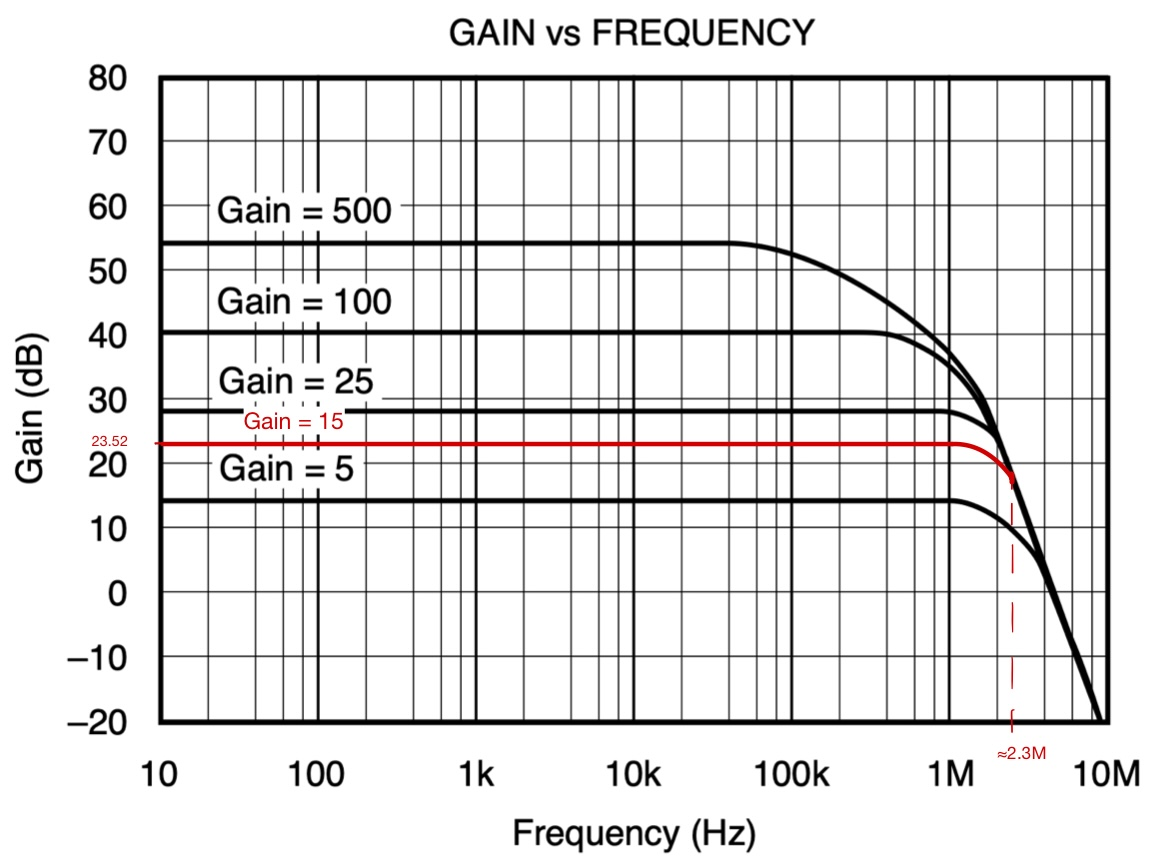
\includegraphics[width=0.5\textwidth]{INA_BW.jpeg}
    \caption{INA331 Bandwidth vs Gain adapted from \cite{INA331}}
    \label{fig:ina_bw}
\end{figure}

The second stage uses a TLV9061 op-amp in an inverting gain configuration. With a GBW of 10 MHz and gain of $A_v=-20$ ($A_{noise}=21$), the expected bandwidth is 476.2 kHz (equation \ref{eq:GBW}). From equations \ref{eq:mag_rollof} and \ref{eq:phase_shift}, an expected -0.094 dB gain reduction and -11.86\textdegree\ phase shift is calculated at 100 kHz. However, this does not need to be calibrated for as an identical gain stage will be used for the current measurement, ensuring that any gain reductions and phase shifts are cancelled out during impedance calculation.

The final circuit for voltage measurement can be seen in figure \ref{fig:vmeas_stage_circuit}.

\begin{figure}[H]
    \centering
    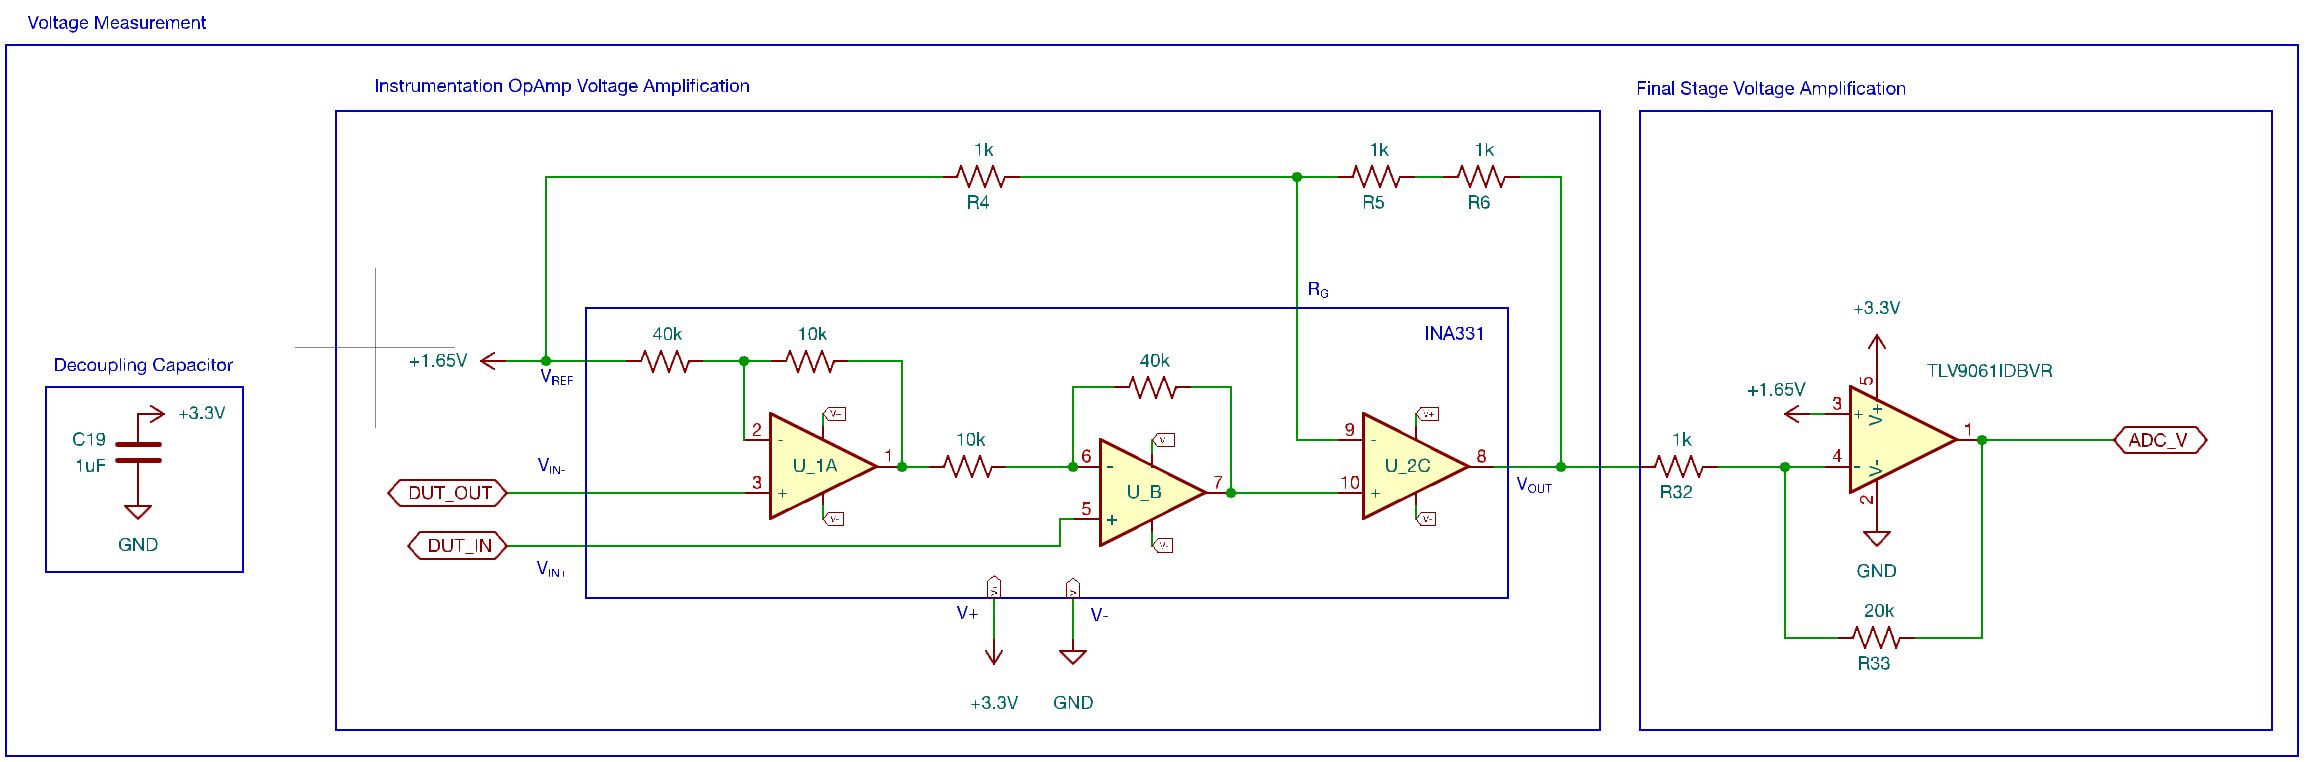
\includegraphics[width=\textwidth]{VMeasSchem.png}
    \caption{Complete Voltage Measurement Stage Circuit}
    \label{fig:vmeas_stage_circuit}
\end{figure}

\subsection{Current Measurement}\label{subsec:design_cur}
The current measurement stage represents the most complex and arguably most important aspect of the analogue frontend. Accurate current measurement across a wide dynamic range is essential for reliable impedance determination.

The architecture consists of three stages: a \ac{TIA} provides the initial current-to-voltage conversion, followed by a \ac{PGA}, then a final inverting gain op-amp stage. This final stage is identical to the second voltage measurement stage, ensuring that gain reductions and phase shifts cancel during impedance calculation.

Based on measurements of the biosensor using the PalmSens4, the expected impedance ranges from \SI{100}{\kilo\ohm} at 1 Hz to \SI{10}{\ohm} at 100 kHz. For a fixed 10 mVpp excitation, this corresponds to a current range from 100 nA to 1 mA, spanning four orders of magnitude. This wide dynamic range drives several critical design requirements.

A fixed-gain amplifier is impractical across this range. High gain would saturate at high currents, whilst low gain would not utilise the full \ac{ADC} range at low currents. Programmable gain is therefore essential. This is achieved through two mechanisms: switchable feedback resistors in the \ac{TIA} and variable gain in the \ac{PGA} stage.

The PGA113 offers gains ranging from 1-200 V/V with a high GBW of 10 MHz and is controlled via SPI. It has a low gain error of $\le0.3\%$ and extremely low noise at $12\text{ nV}/\sqrt{\text{Hz}}$. Combined with the final TLV9061 gain stage (identical to the final voltage measurement stage), this provides variable gain from 20-4000 V/V after the \ac{TIA}. The STM32F303K8 also has an internal \ac{PGA} with an 8 MHz GBW and binary gains from $2^1$ to $2^4$, however it was unclear whether the added flexibility of a second PGA would outweigh the
added noise of an additional gain stage. The PCB was thus designed with a jumper allowing the internal \ac{PGA} to be bypassed. After testing, it was decided that the STM's PGA would not be used.

While the \ac{TIA}'s feedback resistor can be large without affecting the applied signal to the \ac{DUT}, it reduces the bandwidth. If $R_{feedback}$ is too large, the \ac{TIA} experiences significant phase shifts and reduced gain at higher frequencies (referring back to equation \ref{eq:GBW}). Using multiple gain stages distributes the amplification, allowing the \ac{TIA} to use a moderate feedback resistor whilst maintaining adequate bandwidth.

Multiple feedback resistor paths on the \ac{TIA} itself provide additional benefits beyond bandwidth. They enable finer gain segmentation across the input current range, improving measurement precision. The larger feedback resistor handles low currents with maximum resolution, whilst the smaller resistor prevents saturation at high currents. This ensures smooth transitions between gain settings without gaps where currents would be too large for one resistor but too small for the other.

The OPA3S328 is specifically designed for \ac{TIA} applications, with a wide GBW of 40 MHz, 0.2 pA input bias and typical input voltage offset of \SI{10}{\micro\volt}. Importantly, it has integrated switches for switching between feedback resistors. However, the switch on-resistance is non-negligible at 90--125 $\Omega$ and varies with temperature. This produces gain errors and distortion on the \ac{TIA} output. This can be addressed by using the second switch and op-amp integrated into the OPA3S328 package to build a buffered multiplexer. An example of this circuit is shown in Figure \ref{fig:kelvin_sense_tia}. The switch senses the \ac{TIA} output directly at the feedback resistor for each gain, whilst the second op-amp acts as a buffer. The low input bias current of the op-amp ensures negligible voltage drop (a worst case of 1.25 nV), providing an accurate Kelvin sense connection. This eliminates gain error, gain error drift and gain non-linearity due to the switch resistances.

\begin{figure}[]
    \centering
    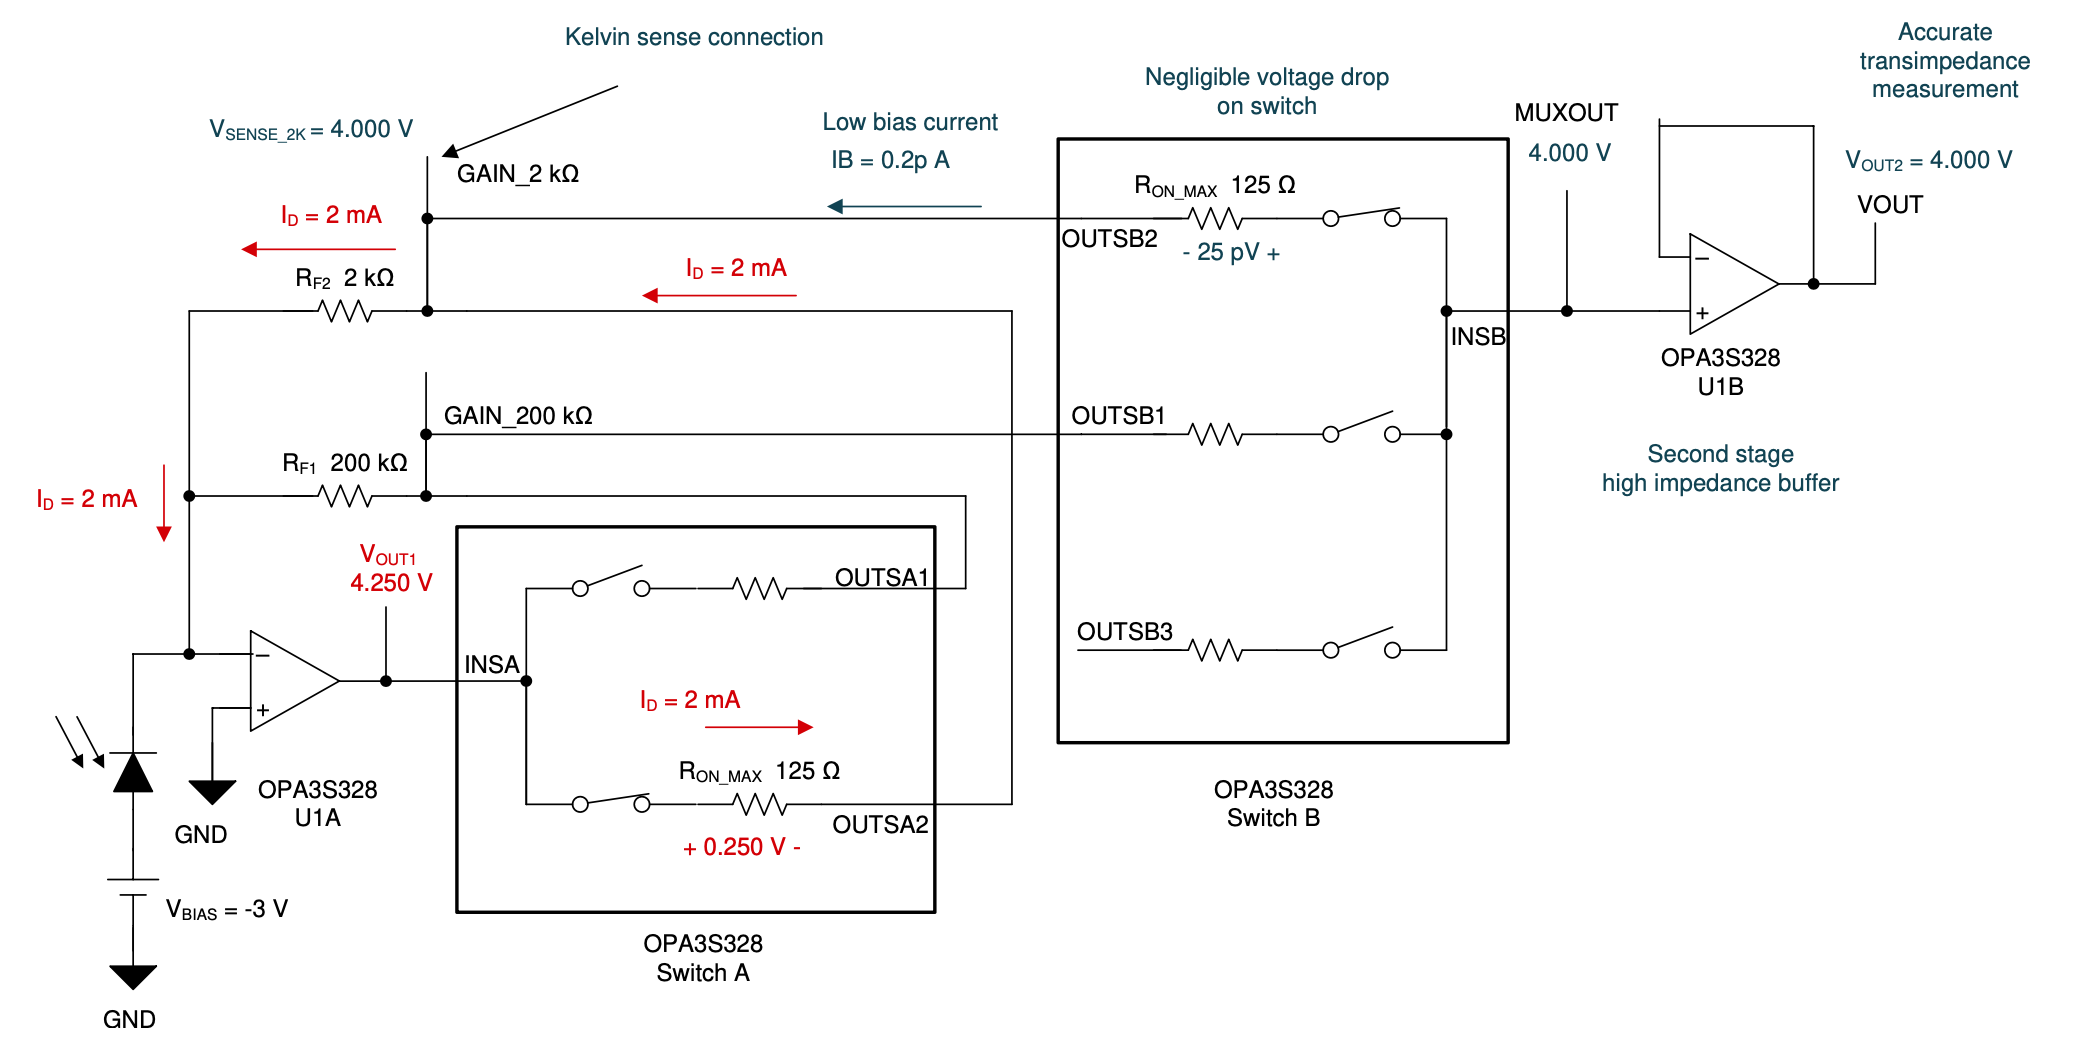
\includegraphics[width=0.8\textwidth]{KelvinSenseTIA.png}
    \caption{Example of Kelvin Sense Switch Connections and High Impedance Buffer\cite{chioyeBuildProgrammableGain2021}}
    \label{fig:kelvin_sense_tia}
\end{figure}

The YBJ variant was chosen due to its 3-way \ac{MUX} over the RGR variant with a 2-way \ac{MUX}, enabling finer gain segmentation and improved measurement precision across the input current range. However, due to the small package size and PCB manufacturing limits (see section \ref{sec:PCB}), only two of the three switches were used.

To maximise the \ac{ADC}'s range even at the smallest current, the larger feedback resistor is designed to deliver 3 Vpp at the maximum \ac{PGA} gain. From equations \ref{eq:tia_1}--\ref{eq:tia_3}, this results in 7.5 k$\Omega$.
\begin{align}
        V_{TIA} &= \frac{3}{4000} = 750 \mu V \label{eq:tia_1}\\
        A_{TIA} &= \frac{750 \mu V}{100 nA} = 7500 V/A \\
        \therefore  R_{f1} &= 7.5 k\Omega \label{eq:tia_3}
\end{align}

The smaller feedback resistor is chosen to give the same overall gain at the maximum \ac{PGA} gain as the larger resistor gives at the minimum \ac{PGA} gain. This ensures a smooth transition between feedback resistors with no currents being too large for the larger feedback resistor but too small for the smaller one. The smaller feedback resistor is calculated to be 200 times smaller at $R_{f2}=37.5 \Omega$. This ensures that the ranges from 50 nA - 20 $\mu$A and 20 $\mu$A - 4 mA are covered respectively, whilst ensuring that the \ac{ADC} input stays between 1.5 - 3 Vpp.

In traditional TIA designs a capacitor is placed in parallel with the feedback resistor to provide sufficient phase margin and ensure stability \cite{StabilizeYourTransimpedance}. These designs are, however intended for use with a photodiode, rather than \ac{EIS}. There are few sources available that discuss the design of a TIA for EIS purposes, where capacitance is what is measured rather than compensated for. These sources do not discuss the necessity of feedback capacitors, thus this has to be derived from theory.

The dominant pole of the open loop response of an op-amp is a function of the GBW and the open loop gain, $A_{OL}$ (equation \ref{eq:fdp}). This determines the -3dB frequency of the open loop transfer function and after this point the gain rolls of at a rate of -20dB/decade. Due to the extremely large open loop gains of modern op-amps (130dB or $3.16 \times 10^6 V/V$ for the OPA3S328), negative feedback is required between the output and inverting input. The amount of the output that is fed back to the input is defined as the feedback factor ($\beta$) and described by equation \ref{eq:fb_factor}. Where $V_{fb}$ is the voltage present at the inverting input of the op-amp and $V_{out}$ the voltage at the output. This negative feedback results in the closed loop gain (equation \ref{eq:acl}) where the loop-gain refers to $A_{OL}\times\beta$ (equation \ref{eq:loop_gain}).

\begin{align}
    \text{Dominant Pole} &= f_{DP} = \frac{\text{GBW}}{A_{OL}} \label{eq:fdp}\\
    \text{Feedback Factor} &= \beta = \frac{V_{fb}}{V_{out}}  \label{eq:fb_factor}\\
    \text{Closed Loop Gain} &= A_{CL} = \frac{A_{OL}}{1 + A_{OL}\beta} \label{eq:acl}\\
    \text{Loop Gain} &= A_{OL}\beta \label{eq:loop_gain}\\
\end{align}

When the loop-gain is -1, equation \ref{eq:acl} simplifies to $A_{CL} = \frac{A_{OL}}{0}$ and the system becomes unstable. This happens when $V_{fb}$ leads or lags $V_{out}$ by 180\textdegree. The phase margin (PM) is thus defined as in equation \ref{eq:pm} and describes how close the system is to a 180\textdegree\ phase shift and instability when the loop gain is at 0dB or 1V/V (the critical point or $f_c$). From equation \ref{eq:aol_at_0db} it is shown that this happens when the magnitude plots of $A_{OL}$ and $\frac{1}{\beta}$ intersect. To ensure stability, the PM should be at least 45\textdegree, with higher values providing more stability at the cost of transient response \cite{StabilizeYourTransimpedance}. The phase margin can be calculated by subtracting the phase of $\frac{1}{\beta(j\omega)}$ from the phase of $A_{OL}(j\omega)$ to get the phase of $A_{OL}\beta(j\omega)$.

\begin{align}
    \text{PM} &= 180^\circ + \varphi_{A_{OL}\beta} \text{ at } |A_{OL}\beta| = 0dB \label{eq:pm} \\
    |A_{OL}\beta| &= 0dB = 1 V/V\\
    \therefore |A_{OL}| &= |\frac{1}{\beta}| \text{ at } f_c \label{eq:aol_at_0db}
\end{align}

\begin{figure}[H]
    \centering
    \begin{minipage}{0.6\textwidth}
        \centering
        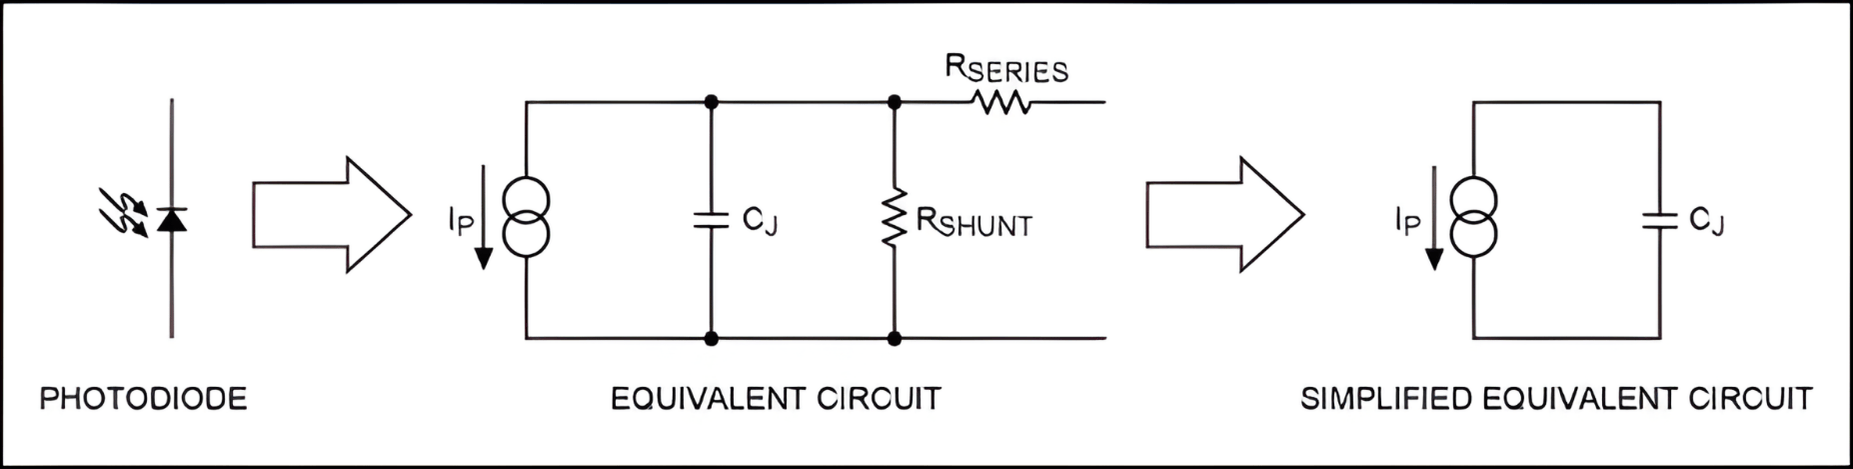
\includegraphics[width=\textwidth]{PhotoDiodeCircuit.png}
        \caption{Photodiode equivalent circuit\cite{StabilizeYourTransimpedance}}
        \label{fig:photodiode}
    \end{minipage}\hfill
    \begin{minipage}{0.4\textwidth}
        \centering
        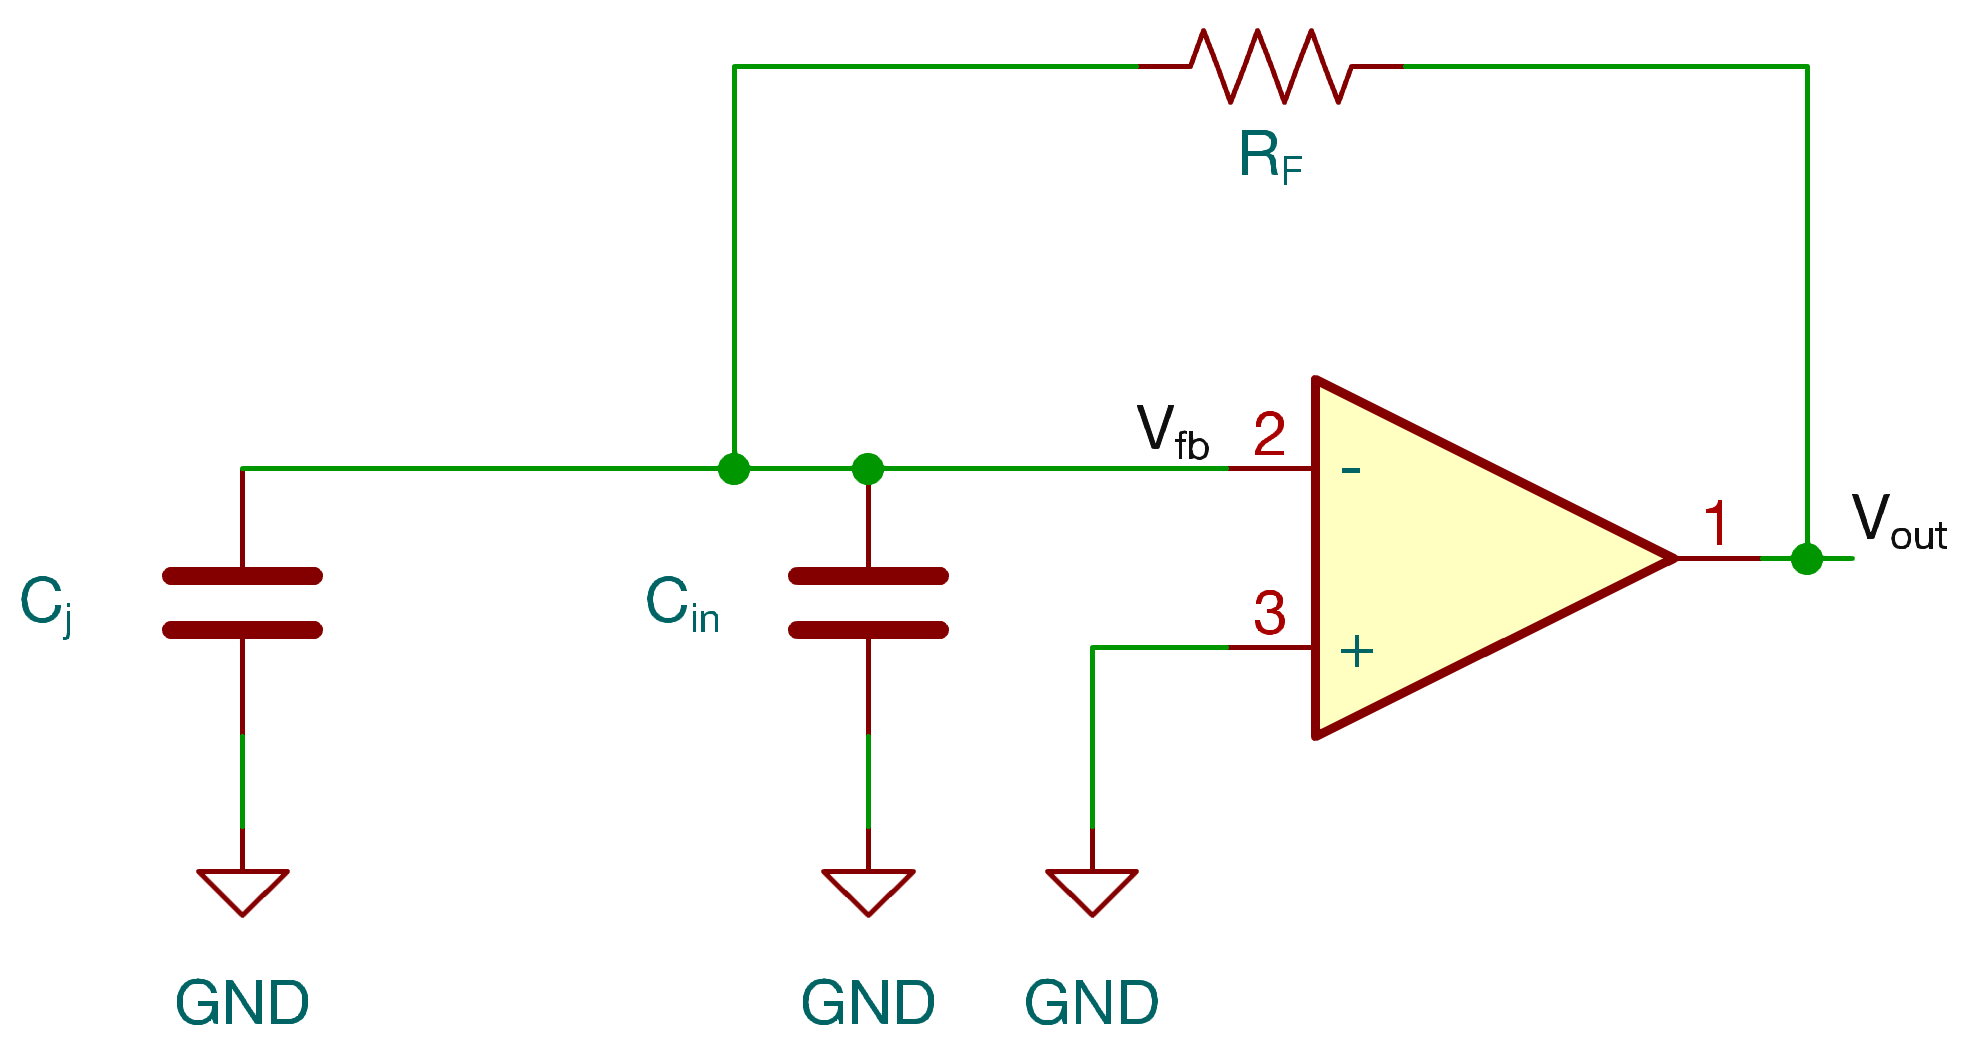
\includegraphics[width=\textwidth]{PhotoTIA.png}
        \caption{Equivalent TIA circuit for photodiodes}
        \label{fig:tia_photo}
    \end{minipage}
\end{figure}

\begin{align}
    C_i &= C_j+C_{in} \\
    \beta (j\omega) &= \frac{X_{c_i}}{R_f + X_{C_i}} = \frac{1}{1+j\omega R_fC_i} \label{eq:photo_beta}\\
    \therefore \frac{1}{\beta(j\omega)} &= 1+j\omega R_fC_i
\end{align}

Figure \ref{fig:photodiode} shows the simplified equivalent circuit of a photodiode, including the junction capacitance ($C_J$). With figure \ref{fig:tia_photo} showing the resulting equivalent circuit model of a TIA for measuring photodiodes, including the input capacitance of the op-amp ($C_{in}$). From this, the feedback factor can be calculated as seen in equation \ref{eq:photo_beta}. The pole in $\beta(j\omega)$, caused by the combined input capacitance, translates to a zero in $\frac{1}{\beta(j\omega)}$. This zero causes the magnitude of $\frac{1}{\beta(j\omega)}$ to increase at a rate of 20dB/decade after the corner frequency (determined by the value of $C_{i}$) and the phase to increase from 0\textdegree to 90\textdegree. The result is a very small phase margin at the critical frequency and instability (as seen in figure \ref{fig:matlab_7.5}). The feedback capacitor in parallel with $R_f$ solves this by adding a pole to $\frac{1}{\beta(j\omega)}$, cancelling out the zero and thus adding phase margin.

\begin{figure}[H]
    \centering
    \begin{minipage}{0.5\textwidth}
        \centering
        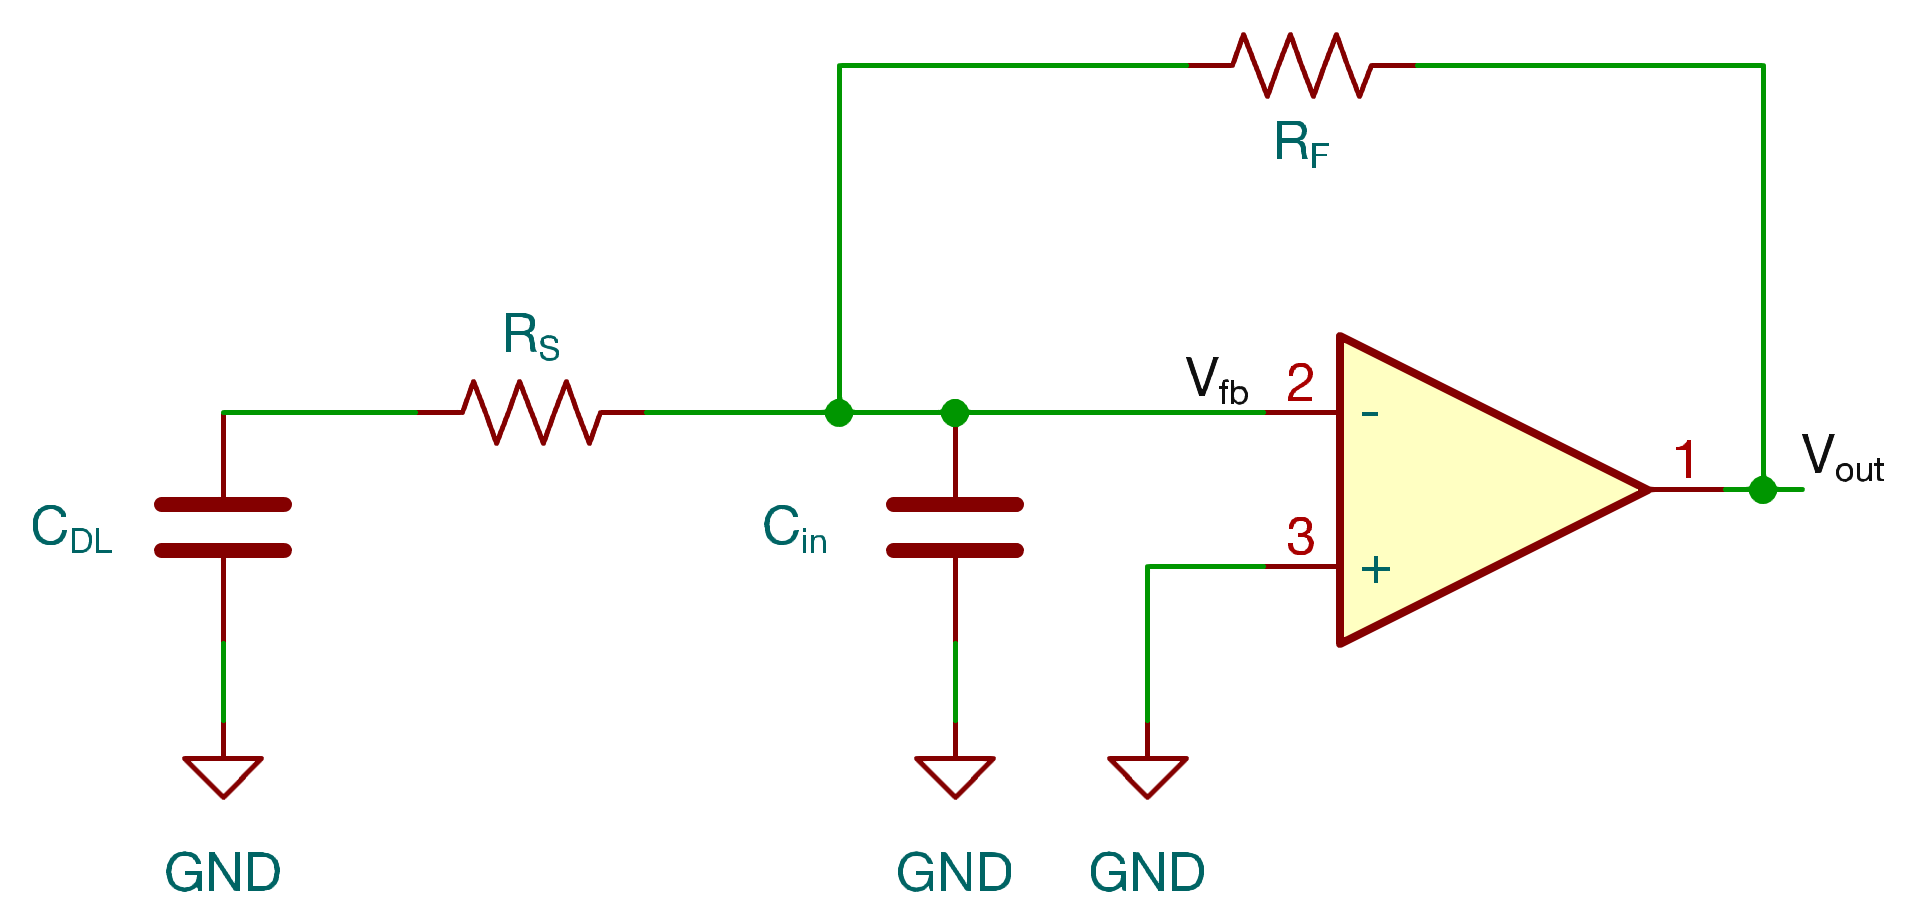
\includegraphics[width=\textwidth]{RandlesSimpleTIA.png}
        \caption{Simplified Randles equivalent TIA circuit with ideal capacitance}
        \label{fig:randles_cdl_tia}
    \end{minipage}\hfill
    \begin{minipage}{0.5\textwidth}
        \centering
        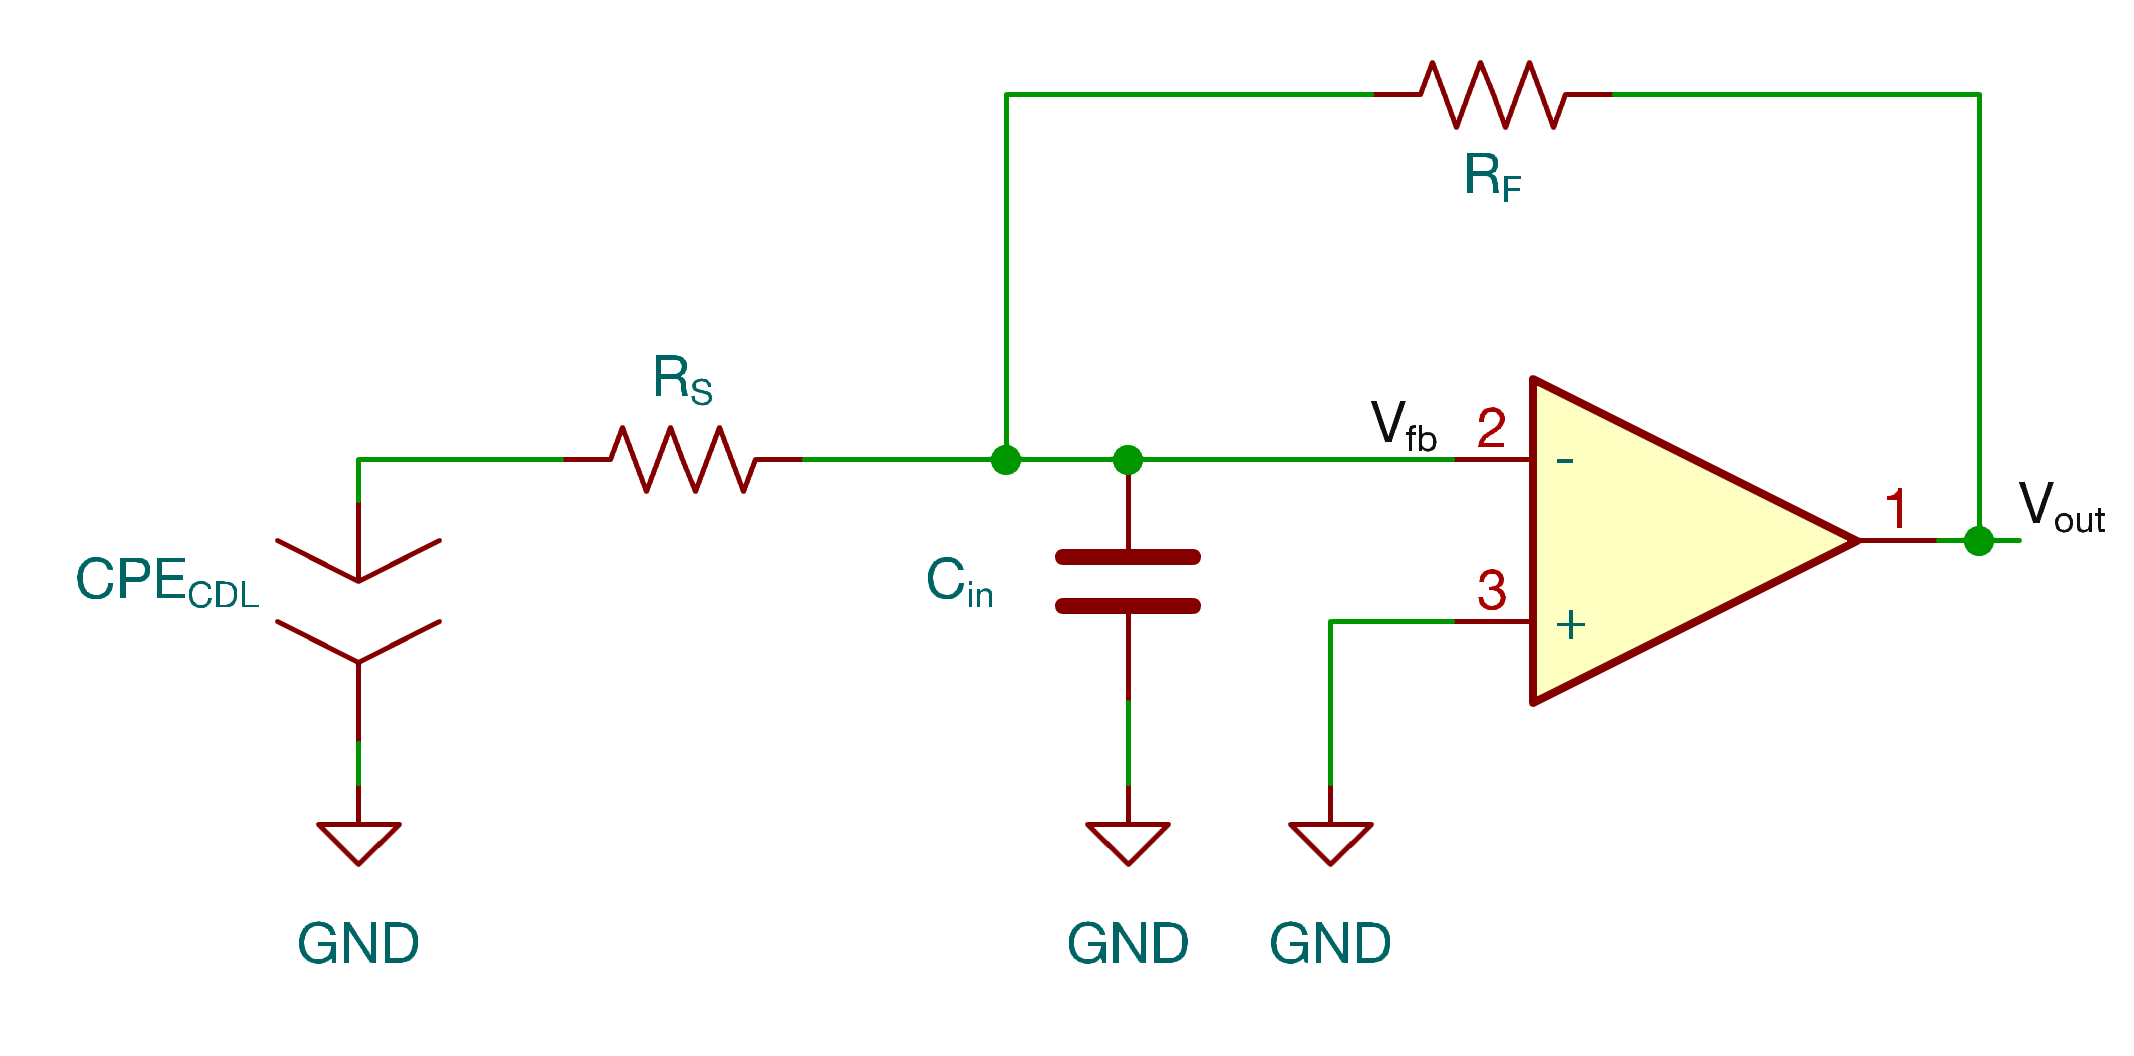
\includegraphics[width=\textwidth]{RandlesTIA.png}
        \caption{Randles equivalent TIA circuit with CPE}
        \label{fig:randles_cpe_tia}
    \end{minipage}
\end{figure}

Simplified Randles Circuit with Ideal Capacitance:
\begin{align}
    Z_{in} &= (R_S + X_{C_{DL}}) || X_{C_{in}} \label{eq:simple_zin}\\
    \beta (j\omega) &= \frac{Z_{in}}{R_f + Z_{in}} \label{eq:simple_beta} \\
    \therefore \frac{1}{\beta(j\omega)} &= 1 + \frac{R_f}{Z_{in}} \nonumber\\
    &= 1 + \frac{R_f}{(R_S + X_{C_{DL}}) || X_{C_{in}}}
\end{align}
Full Randles Circuit with CPE:
\begin{align}
    Z_{CPE} &= \frac{1}{T(j\omega)^{\alpha}} \\
    Z_{in} &= (R_S + Z_{CPE}) || X_{C_{in}} \\
    \beta (j\omega) &= \frac{Z_{in}}{R_f + Z_{in}} \label{eq:randles_beta}\\
    \therefore \frac{1}{\beta(j\omega)} &= 1 + \frac{R_f}{Z_{in}} \nonumber\\
    &= 1 + \frac{R_f}{(R_S + Z_{CPE}) || X_{C_{in}}}
\end{align}

However, the equivalent Randles circuit model of a biosensor differs fundamentally from the model of a photodiode due to the series resistance $R_s$. Figures \ref{fig:randles_cpe_tia} and \ref{fig:randles_cdl_tia} show the equivalent TIA circuits for a non-faradaic Randles circuit and a simplified model using an ideal capacitance ($C_{dl}$) instead of the \ac{CPE} by approximating $T=C_{dl}$ and $\alpha=1$. For the simplified model, the input impedance and feedback factor can be calculated as seen in equations \ref{eq:simple_zin} - \ref{eq:simple_beta}. The full Randles non faradaic equivalent circuit results in \ref{eq:randles_beta}. The series resistance and double layer capacitance of the biosensor was estimated using PS Trace and values for input capacitance, open loop gain and gain bandwidth were read from the OPA3S328 datsheet. A MatLab script was then used to calculate the $\frac{1}{\beta(j\omega)}$ transfer function and loop gain of the system. Similairly the series resistance, $T$ and $\alpha$ values were estimated for the Randles circuit using circuit fitting in PS Trace and plotted in MatLab. The response of the equivalent photodiode model was also plotted using the constant $C_{DL}$ as the parasitic junction capacitance. Table \ref{tab:stability_params} shows the estimated circuit paramaters and figures \ref{fig:matlab_7.5} and \ref{fig:matlab_37.5} shows the resulting responses. Table \ref{tab:matlab_results} lists the calculated critical frequencies and phase margins.

\begin{figure}[H]
    \centering
    \begin{subfigure}[b]{0.5\textwidth}
        \centering
        \includegraphics[width=\textwidth]{MatLabBeta_37,5.png}
        \caption{$\frac{1}{\beta(j\omega)}$ frequency response}
        \label{fig:matlab_beta_37.5}
    \end{subfigure}\hfill
    \begin{subfigure}[b]{0.5\textwidth}
        \centering
        \includegraphics[width=\textwidth]{MatLabLG_37,5.png}
        \caption{Loop Gain frequency response}
        \label{fig:matlab_cl_37.5}
    \end{subfigure}
    \caption{Calculated frequency responses for $R_F=37.5\Omega$}
    \label{fig:matlab_37.5}
\end{figure}
\begin{figure}[H]
    \centering
    \begin{subfigure}[b]{0.5\textwidth}
        \centering
        \includegraphics[width=\textwidth]{MatLabBeta_7500.png}
        \caption{$\frac{1}{\beta(j\omega)}$ frequency response}
        \label{fig:matlab_beta_7.5}
    \end{subfigure}\hfill
    \begin{subfigure}[b]{0.5\textwidth}
        \centering
        \includegraphics[width=\textwidth]{MatLabLG_7500.png}
        \caption{Loop Gain frequency response}
        \label{fig:matlab_cl_7.5}
    \end{subfigure}
    \caption{Calculated frequency responses for $R_F=7.5k\Omega$}
    \label{fig:matlab_7.5}
\end{figure}

From these plots, the difference between the photodiode and biosensor circuits become clear. At low frequencies the simplified biosensor circuit closely follows the response of the photodiode. \rephrase{This is due to the zero caused by the capacitance dominating the response ($X_{C_{DL}}>>R_S$) and thus the equivalent circuits of the photodiode and Randles circuit are near identical.} However, at higher frequencies $R_S$ becomes much larger than $X_{C_{DL}}$ and the responses start to diverge. The dominance of $R_S$ at higher frequencies ensure that ample phase margin is achieved by the critical frequency. The full Randles non-faradaic circuit model provides a more accurate representation of the biosensor TIA circuit and diverges earlier than the simplified circuit due to the \ac{CPE}. This confirms that ample phase margin is available at both $R_f=37.5\Omega$ and $R_f=7.5k\Omega$, meaning that no feedback capacitors are needed. At extremely large values of $R_F$ the phase margin reduces, and the system can become unstable ($R_f>40k\Omega$ for this circuit). Since adding compensation capacitors reduces the bandwidth of the TIA \cite{StabilizeYourTransimpedance}, it is not recommended for biosensing TIA circuits, except in cases of extremely high feedback resistor values.

\begin{table}[H]
    \centering
    \begin{minipage}{0.3\textwidth}
        \centering
        \caption{Circuit Parameters}
        \label{tab:stability_params}
        \begin{tabular}{ll}
            \hline
            \textbf{Parameter} & \textbf{Value} \\
            \hline
            \multicolumn{2}{l}{\textit{CPE Randles Circuit}} \\
            $R_S$ & \SI{8.975}{\ohm} \\
            $T$ & \SI{6.993e-6}{} \\
            $\alpha$ & 0.785 \\
            $C_{in}$ & \SI{4.0}{\pico\farad} \\
            \hline
            \multicolumn{2}{l}{\textit{Constant C Randles Circuit}} \\
            $R_S$ & \SI{12.3}{\ohm} \\
            $C_{DL}$ & \SI{1436.0}{\nano\farad} \\
            $C_{in}$ & \SI{4.0}{\pico\farad} \\
            \hline
            \multicolumn{2}{l}{\textit{Photodiode Equivalent}} \\
            $C_i$ & \SI{1436.0}{\nano\farad} \\
            \hline
        \end{tabular}
    \end{minipage}\hfill
    \begin{minipage}{0.6\textwidth}
        \centering
        \caption{Stability Analysis Results}
        \label{tab:matlab_results}
        \begin{tabular}{lccc}
            \hline
            \textbf{Configuration} & $f_c$ & \textbf{PM} & \textbf{Status} \\
             & \textbf{(kHz)} & \textbf{(\textdegree)} & \\
            \hline
            \multicolumn{4}{l}{\textit{$R_f = \SI{7.5}{\kilo\ohm}$}} \\
            Constant C Randles & 65.83 & 82.2 & Stable \\
            Photodiode & 24.22 & 0.1 & Unstable \\
            CPE Randles & 64.22 & 63.8 & Stable \\
            \hline
            \multicolumn{4}{l}{\textit{$R_f = \SI{37.5}{\ohm}$}} \\
            Constant C Randles & 9840.03 & 89.8 & Stable \\
            Photodiode & 343.77 & 0.5 & Unstable \\
            CPE Randles & 7725.81 & 86.3 & Stable \\
            \hline
        \end{tabular}
    \end{minipage}
\end{table}

The final current measurement circuit is shown in Figure \ref{fig:imeas_stage_circuit}.

\begin{figure}[H]
    \centering
    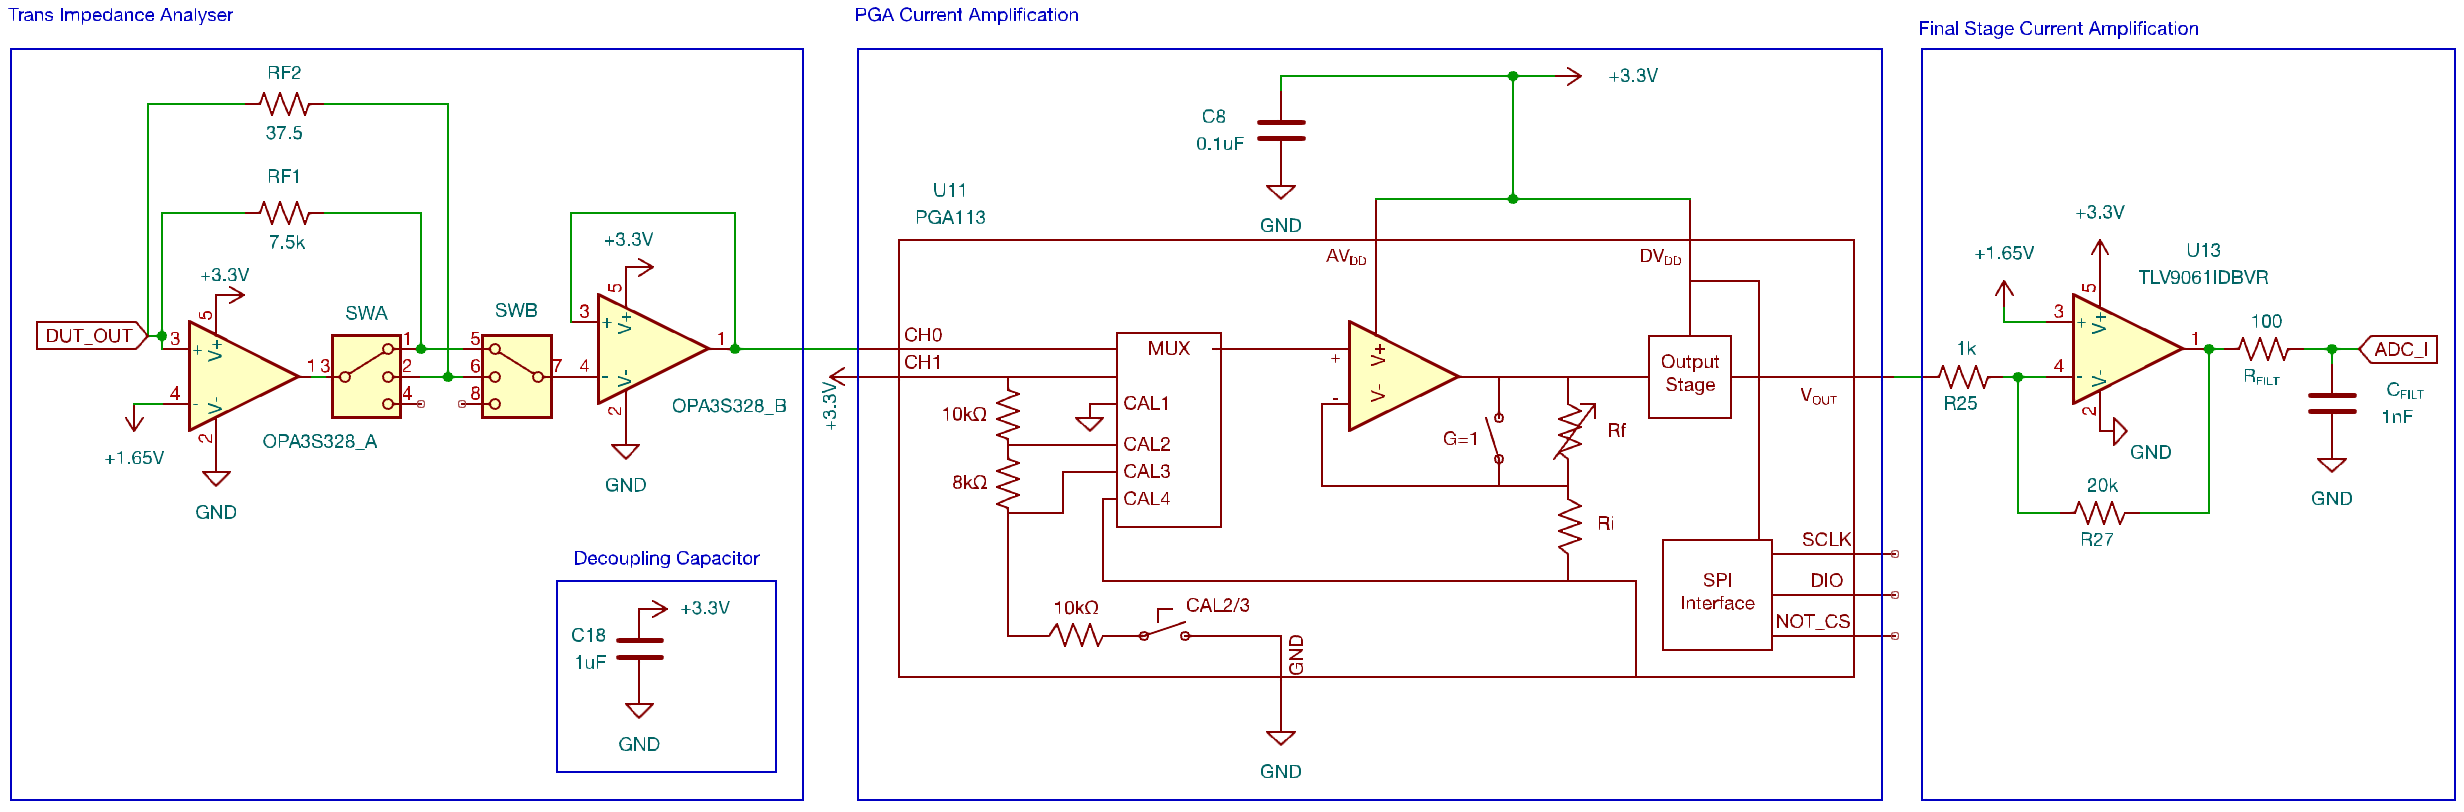
\includegraphics[width=\textwidth]{IMeasSchem.png}
    \caption{Complete Current Measurement Stage Circuit}
    \label{fig:imeas_stage_circuit}
\end{figure}

\subsection{DUT}
The design and manufacture of biosensors are outside the scope of this project. The biosensors described in \cite{ebrahimDevelopmentBiosensorEarly2023} were used for this project, however the system could easily be adapted to work with other capacitive biosensors. To ensure ease-of-use, a method of interfacing with the biosensors that is simple and reliable needed to be developed. Spring-loaded battery connectors were used as they allow the DUT to be easily slid in and out of the device when combined with a 3d printed \rephrase{enclosure}.

\todo{Insert 3d model of connectors, dut and 3d print.}
\subsection{Multiplexer}
Two approaches towards multiplexing were considered. One approach is to have multiple excitation sources and measurement stages, allowing for simultaneous measurements of all \acp{DUT}. \rephrase{This approach has the advantage of speeding up the measurement process, while allowing each \ac{DUT} to have electronics dedicated to its measurement range.} The major disadvantages to this approach is complexity and cost.

Another approach is re-using the same excitation and measurement circuitry, by switching the input and outputs between the \acp{DUT}. This reduces the cost and complexity, but is reliant on having a reliable switching mechanism that does not impact the measurements.

Ultimately the best approach was using a single set of excitation and measurement circuitry, multiplexed in order to measure \acp{DUT} sequentially. The cost reductions of this approach outweighs the increased measurement time as no user input is required between \ac{DUT} measurements.

Various options for multiplexers were considered including dedicated analogue multiplexers (MUX ICs), op-amp based multiplexers and relays. Dedicated analogue multiplexers consist of a collection of analogue switches. They typically use CMOS technology, resulting in compact integration and fast switching speeds. Modern analogue switches are available with very low on-resistance ($<1\Omega$) and a high degree of flatness \cite{SelectingRightCMOS}. However, leakage currents are inherent to these solid-state devices and can corrupt low-current signals, especially in the nanoampere range \cite{SelectingRightCMOS}. 

Op-amp-based multiplexers such as seen in Figure \ref{fig:opamp_mux} provide buffering and impedance matching, which make them ideal for multiplexing voltage signals, but the buffering also make them unsuitable for use with current signals.

\begin{figure}[H]
    \centering
    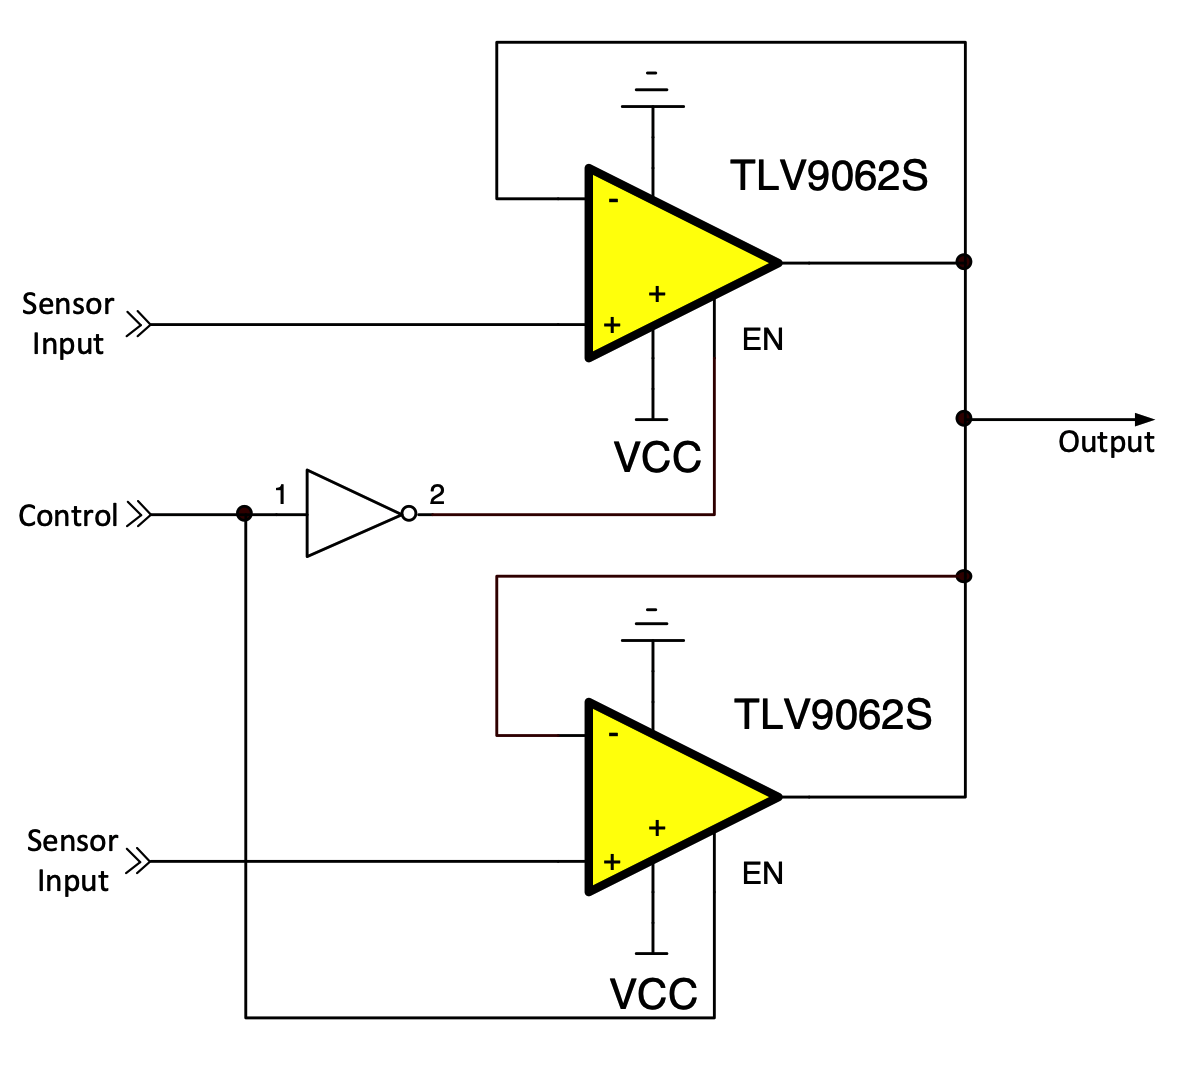
\includegraphics[width=0.4\textwidth]{OpAmpMux.png}
    \caption{Op-amp based multiplexer circuit \cite{Sboa311a}}
    \label{fig:opamp_mux}
\end{figure}

Signal relays, in contrast, use electromechanical contacts to physically open or close signal paths, offering near-zero leakage current and extremely low, stable contact resistance that is independent of signal voltage and temperature. This physical isolation and connection ensures that the measured current accurately reflects the biosensor response. While relays are slower to switch and larger than solid-state alternatives, their switching speed is more than sufficient for switching between sensors.

The TXS2-L2-3V DPDT latching signal relay was chosen due to its small size, low operating current (23.3 mA) and high mechanical lifetime (Minimum 200 000 operations). The major concern of a mechanical relay is the mechanical wear, however at an assumed 2 actuations per measurement and 50 measurements a day, the relays are expected to last more than 5 years. Utilising the DPDT topology of the relay, they can be configured in a tree pattern, allowing for 4 DUT's to be switched using 3 relays as seen in figure \ref{fig:relay_topology}. 

Despite the low operating current, a driver circuit is still needed to power the relay from a microcontroller GPIO. This consists of a lowside NPN transistor and a flyback diode to protect against voltage spikes when the coil is switched off. The final circuit can be seen in figure \ref{fig:relay_circuit}

\begin{figure}[H]
    \centering
    \begin{minipage}{0.35\textwidth}
        \centering
        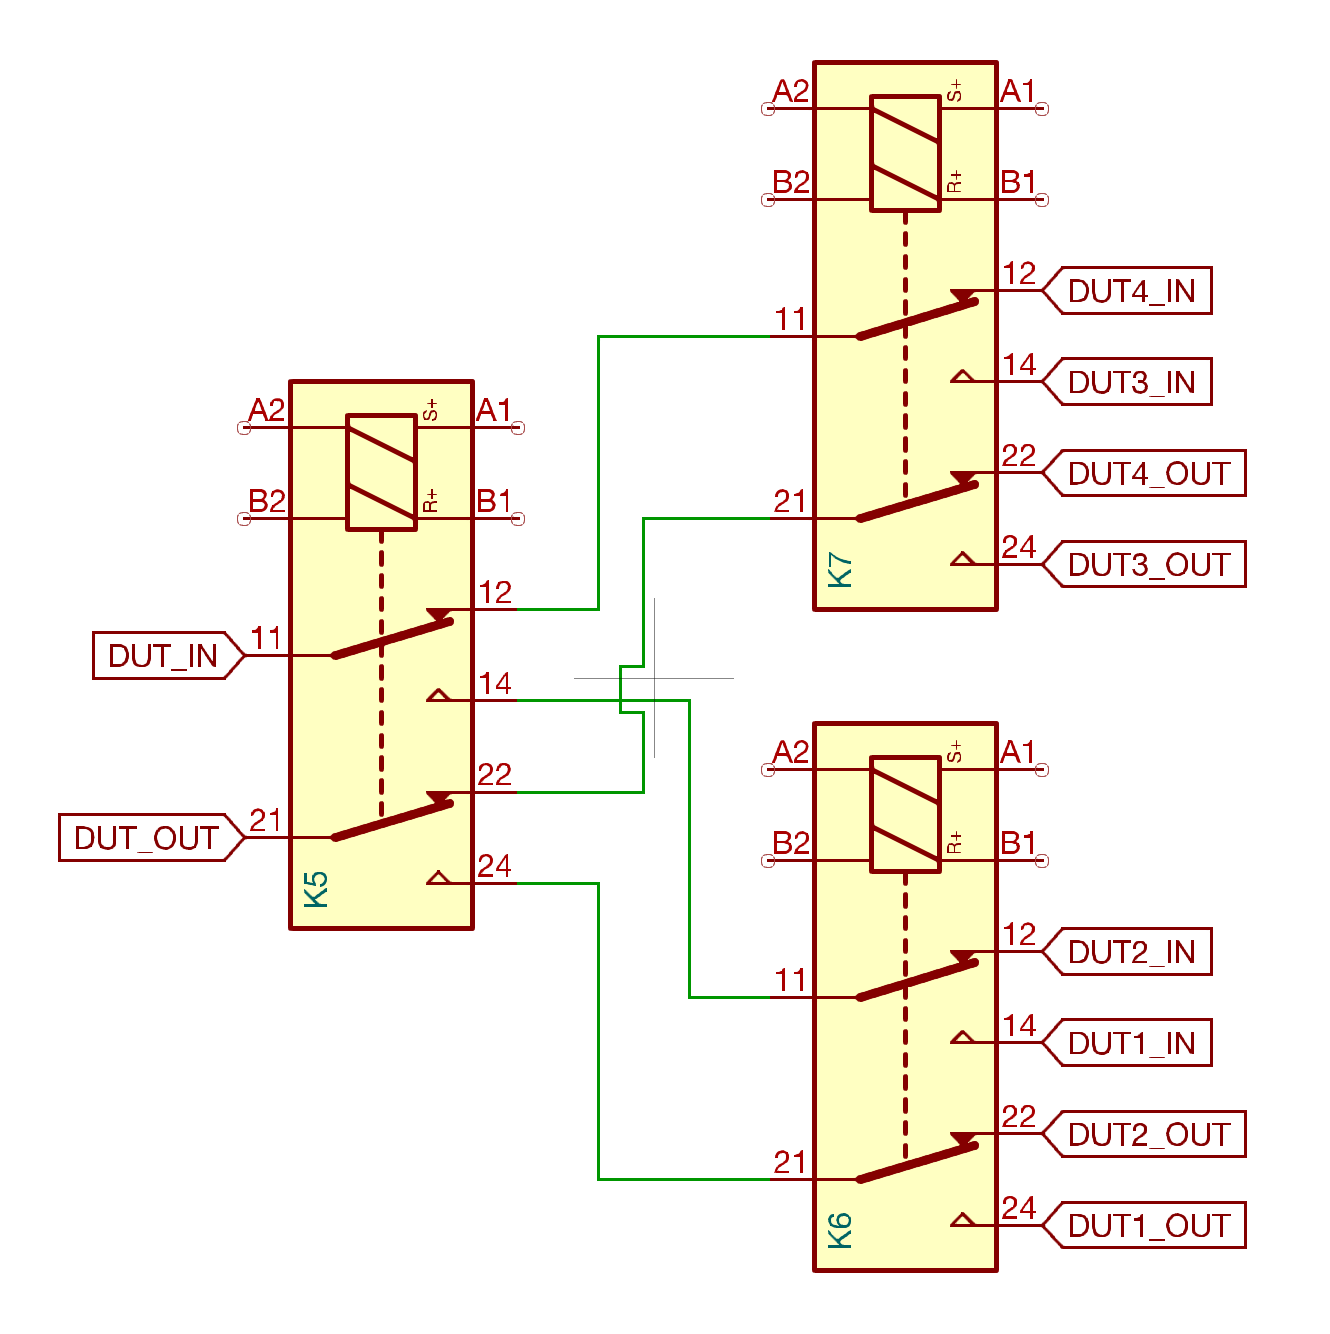
\includegraphics[width=\textwidth]{RelayTopologySchem.png}
        \caption{Relay Multiplexer Topology for 4 DUT's}
        \label{fig:relay_topology}
    \end{minipage}\hfill
    \begin{minipage}{0.6\textwidth}
        \centering
        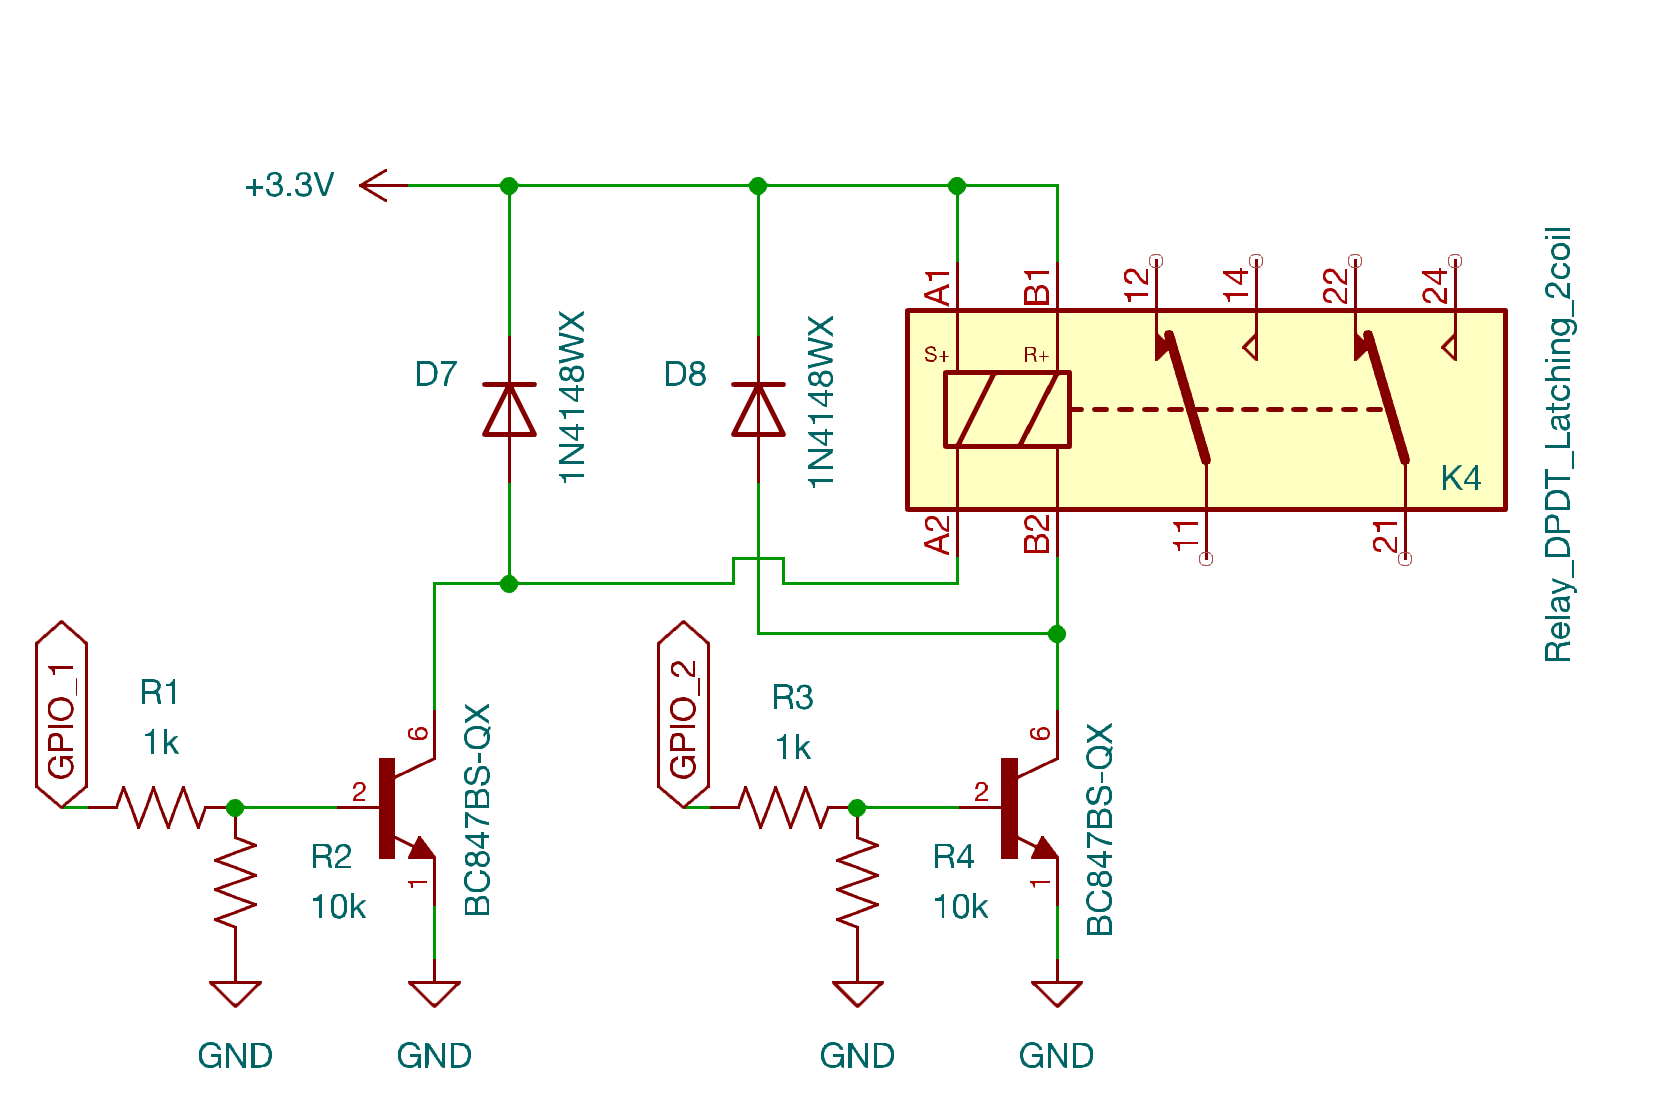
\includegraphics[width=\textwidth]{RelayDriverSchem.png}
        \caption{Relay Driver Circuit for one relay}
        \label{fig:relay_circuit}
    \end{minipage}
\end{figure}

\subsection{Power Circuitry}
\rephrase{With portability in mind, a battery is a requirement for the system.} It was decided that the most cost-effective approach would be to utilise a microcontroller with built-in LiPo charging circuitry instead of a dedicated charging circuit as this is commonly available in many ESP32 boards. \rephrase{The 3.3V rail from the ESP will then be used to power the rest of the system.} 

As mentioned in Section \ref{subsec:design_excitation}, a 1.65V reference is needed for the analogue circuitry. Due to the small amplitude of the excitation signal, it needs to be highly accurate and stable. This was done through the use of a matched resistor array and a op-amp buffer. Using a resistor array ensures that our reference is the exact midpoint of the supply voltage despite any tolerances in the precise resistor value, while the op-amp buffers this output to avoid loading the resistor array and causing a voltage drop. Choosing a too large resistor value risks a slightly uneven voltage drop due to the input bias current of the op-amp buffer, on the other hand, a lower value increases the static current draw and power consumption. $1k\Omega$ was chosen as a balance between these tradeoffs.

\begin{figure}[H]
    \centering
    \begin{minipage}{0.35\textwidth}
        \centering
        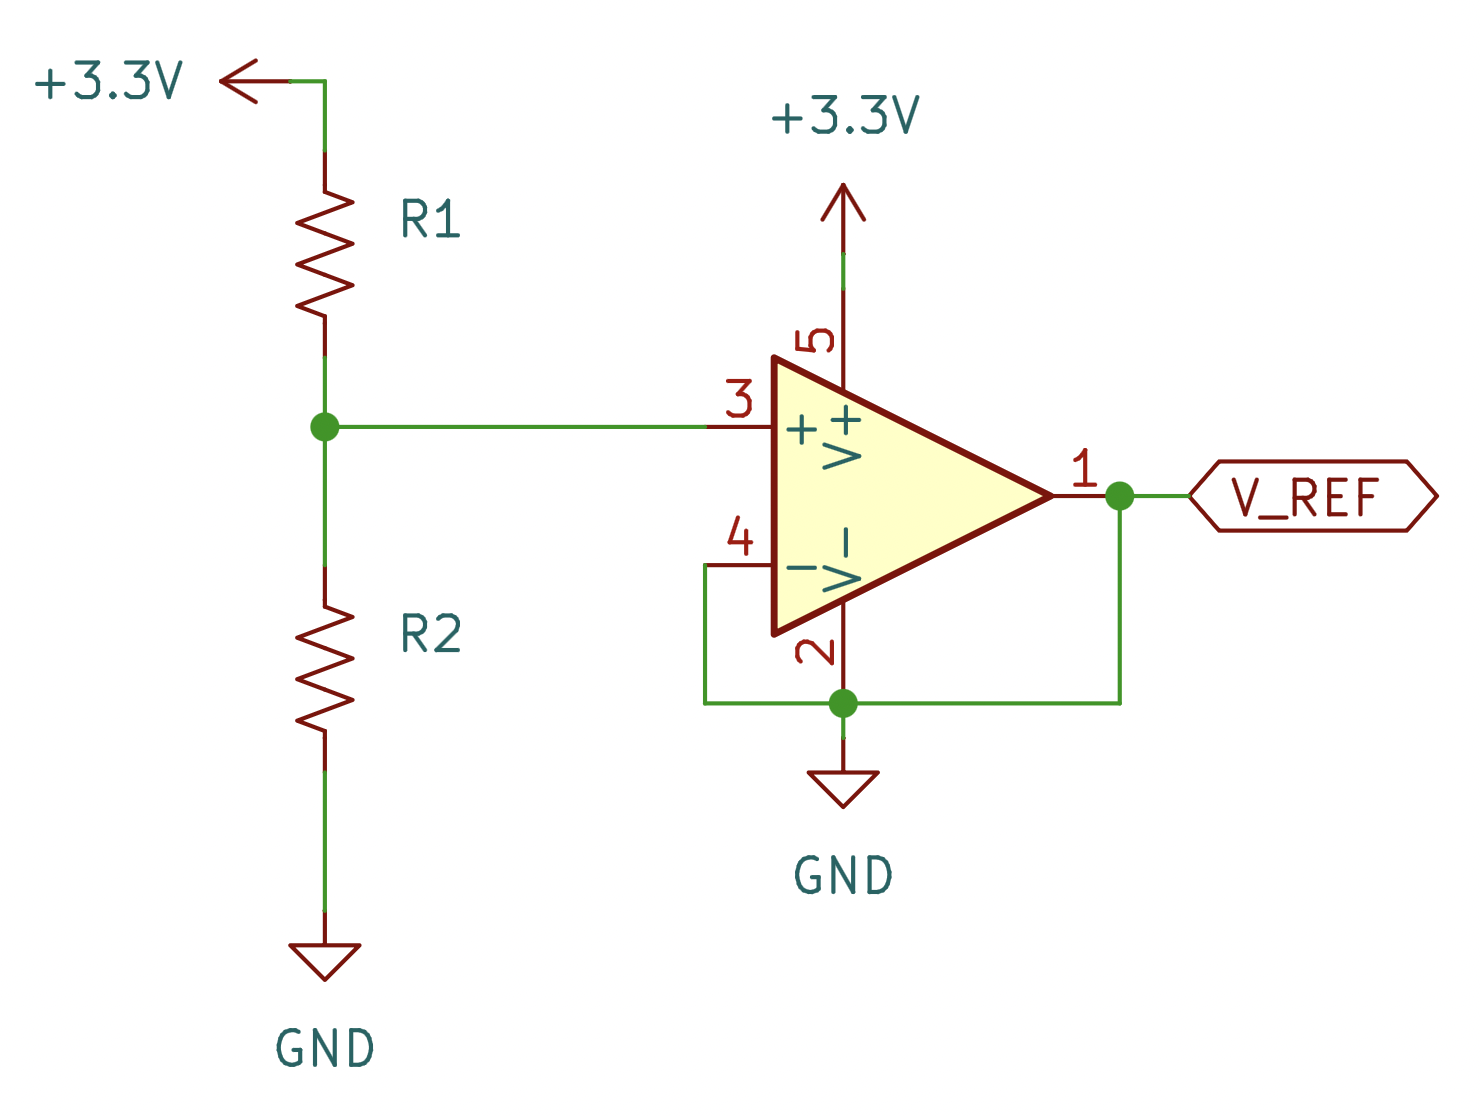
\includegraphics[width=\textwidth]{Vground.png}
        \caption{\newline Virtual ground reference circuit}
        \label{fig:virtual_ground}
    \end{minipage}\hfill
    \begin{minipage}{0.6\textwidth}
        \centering
        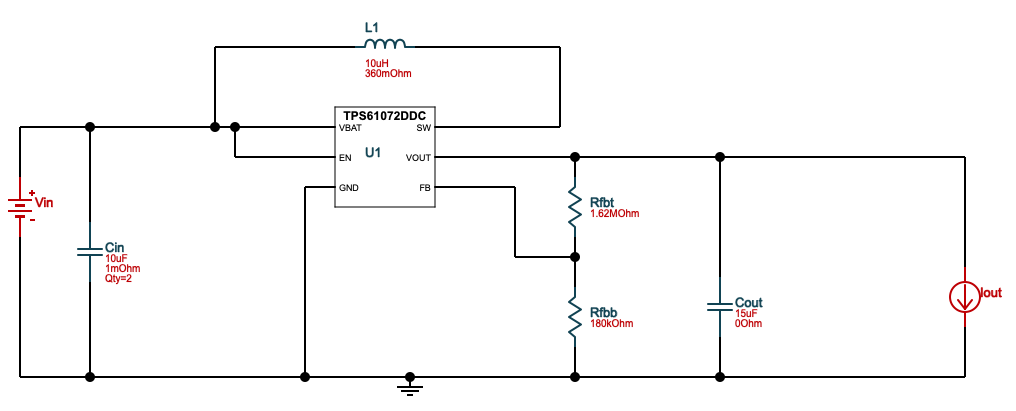
\includegraphics[width=\textwidth]{5V_Reg.png}
        \caption{5V boost converter circuit}
        \label{fig:5V_reg}
    \end{minipage}
\end{figure}

The LTC1069 AA-Filter requires a 5V supply voltage. A 3.3V to 5V boost circuit was designed around the TPS61072 boost regulator using the TI WeBench power supply design tool \cite{WEBENCHCIRCUITDESIGNERDesignTool}, ensuring a stable and efficient circuit as seen in figure \ref{fig:5V_reg}. 

\subsection{Signal Processing}

\subsection{User Interface}
\todo{Fill in once GUI is actually done}
\todo{Talk about flexibility of having both physical buttons and display aswell as web ui, allowing both standalone use and use with either computer, tablet or cell phone, ensuring versatility across environments}

\section{Circuit Simulation}

\subsection{Biosensor}
Despite the widespread use of \acp{CPE} in electrical simulations, the SPICE family of simulators lack a native CPE element. \needscite{There are a variety of approaches to modelling \acp{CPE} such as Laplace transform, Fourier theory or using a network of resistors and capacitors.} \cite{wilsonSimulatingFractionalCapacitors2023} builds on existing approaches to modelling a CPE using a combination of resistors and capacitors (such as \needscite{Add references from wilson}), by using an array of parallel RC elements as seen in Fig \ref{fig:RC_CPE}. The branches form a theoretically infinite geometric progression of characteristic frequencies \cite{wilsonSimulatingFractionalCapacitors2023}, however characteristic frequencies above and below the frequency range of interest are approximated using a single capacitor and resistor respectively. \cite{wilsonSimulatingFractionalCapacitors2023} provides MatLab code that calculates the R and C values of all the branches and this was used to model a CPE element matching the biosensor in LTSpice. Figure \ref{fig:cpe_sim} shows that the CPE model does indeed exhibit a constant phase across the measurement range of interest (1Hz-100kHz) and figure \ref{fig:biosensor_sim} shows the simulated response of the biosensor including $R_S$. Comparing this to the PalmSens measurements (figure \ref{fig:ps_ide}) shows that this model serves as a fairly accurate representation of the \ac{DUT} for simulation purposes.

\subsection{Excitation stage}
For the simulation of the excitation stage, a sample-and-hold block was used to mimic the DAC at varying sample rates. LTSpice has no included components to simulate a raised cosine filter, thus a FIR filter block from \cite{FilterManual} with a raised cosine response and $\beta = 1$ was used. Comparing the simulated frequency response with the LTC1069-7 datasheet (Figures \ref{fig:lt_aa_freq} and \ref{fig:ltc_aa_freq}) for cutoff frequencies of 10kHz and 100kHz, the overall magnitude response is a good approximation, despite some differences at high levels of attenuation ($<-50dB$). The simulated phase response, however is non-linear which does not match the LTC1069-7, but this will not impact the overall system simulation as the DUT is being excited at a single frequency. The TLV9061, INA331 and OPA3s328 PSpice models were obtained from TI and adapted to work in LT Spice. The TLV9061 was used for the attenuation stage.

\begin{figure}[H]
    \centering
    \begin{subfigure}[b]{0.48\textwidth}
        \centering
        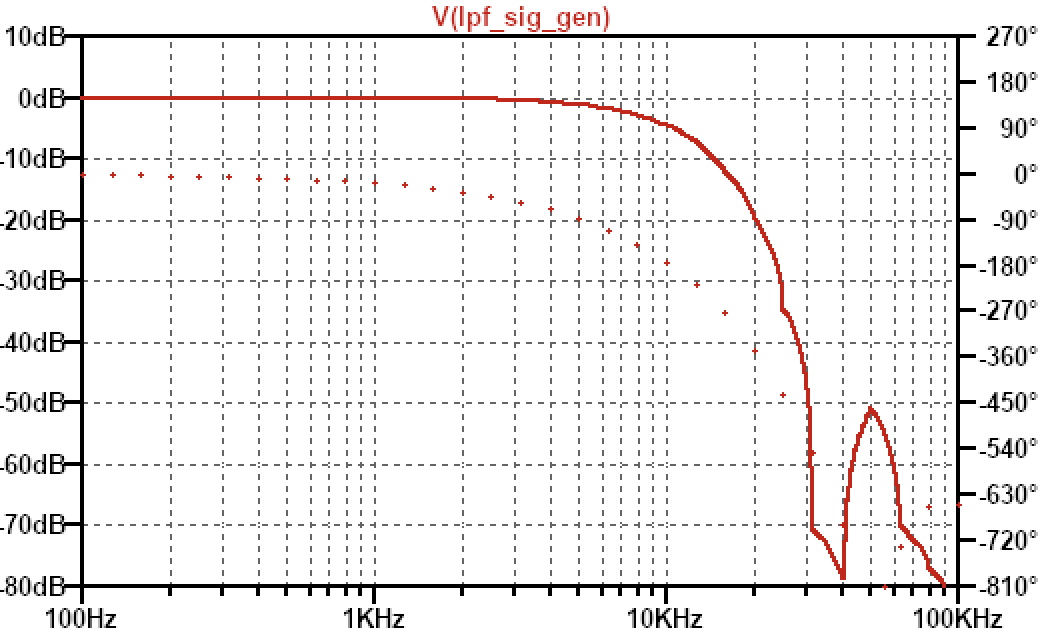
\includegraphics[width=\textwidth]{FIR_10k.png}
        \caption{10kHz cutoff frequency}
        \label{fig:fir_10k}
    \end{subfigure}\hfill
    \begin{subfigure}[b]{0.48\textwidth}
        \centering
        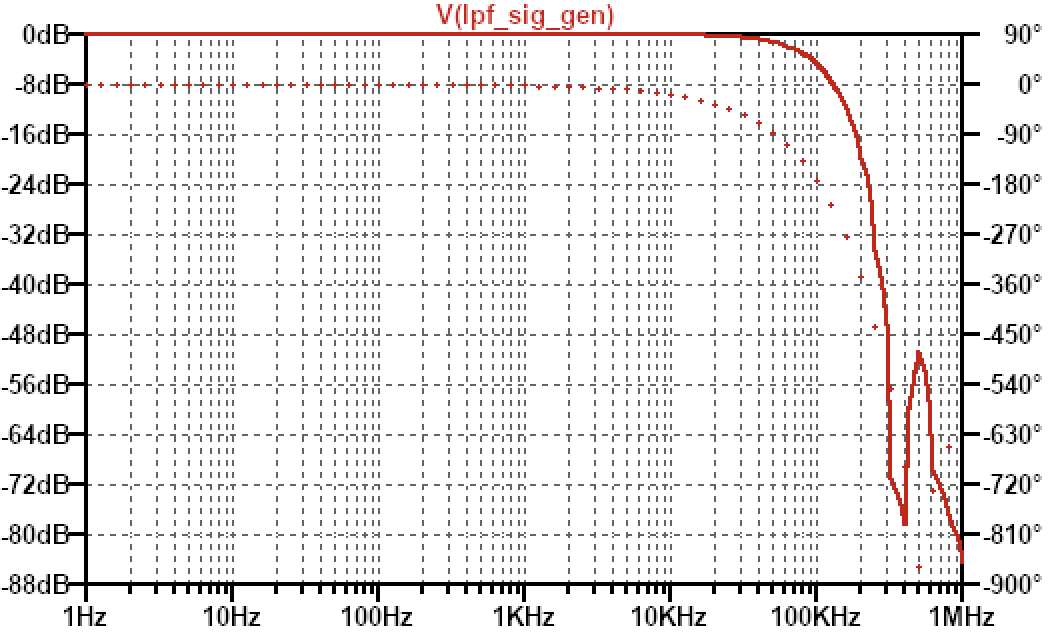
\includegraphics[width=\textwidth]{FIR_100k.png}
        \caption{100kHz cutoff frequency}
        \label{fig:fir_100k}
    \end{subfigure}
    \caption{Simulated FIR filter frequency responses}
    \label{fig:lt_aa_freq}
\end{figure}

\begin{figure}[H]
    \centering
    \begin{subfigure}[b]{0.4\textwidth}
        \centering
        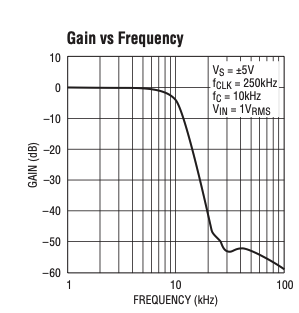
\includegraphics[width=\textwidth]{LTC_10k.png}
        \caption{10kHz cutoff frequency}
        \label{fig:ltc_10k}
    \end{subfigure}\hfill
    \begin{subfigure}[b]{0.4\textwidth}
        \centering
        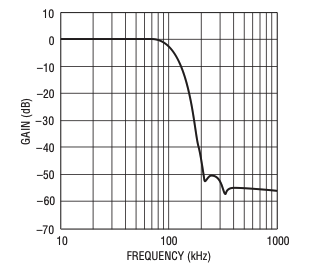
\includegraphics[width=\textwidth]{LTC_100k.png}
        \caption{100kHz cutoff frequency}
        \label{fig:ltc_100k}
    \end{subfigure}
    \caption{LTC1069-7 datasheet frequency responses}
    \label{fig:ltc_aa_freq}
\end{figure}

Figure \ref{fig:dac_filtering} shows a 10kHz signal with 32x oversampling generated by the DAC before and after passing through the AA-filter and after being attenuated. Figure \ref{} shows current through the simulated DUT resulting from this signal.

\begin{figure}[H]
    \centering
    \begin{subfigure}[b]{0.48\textwidth}
        \centering
        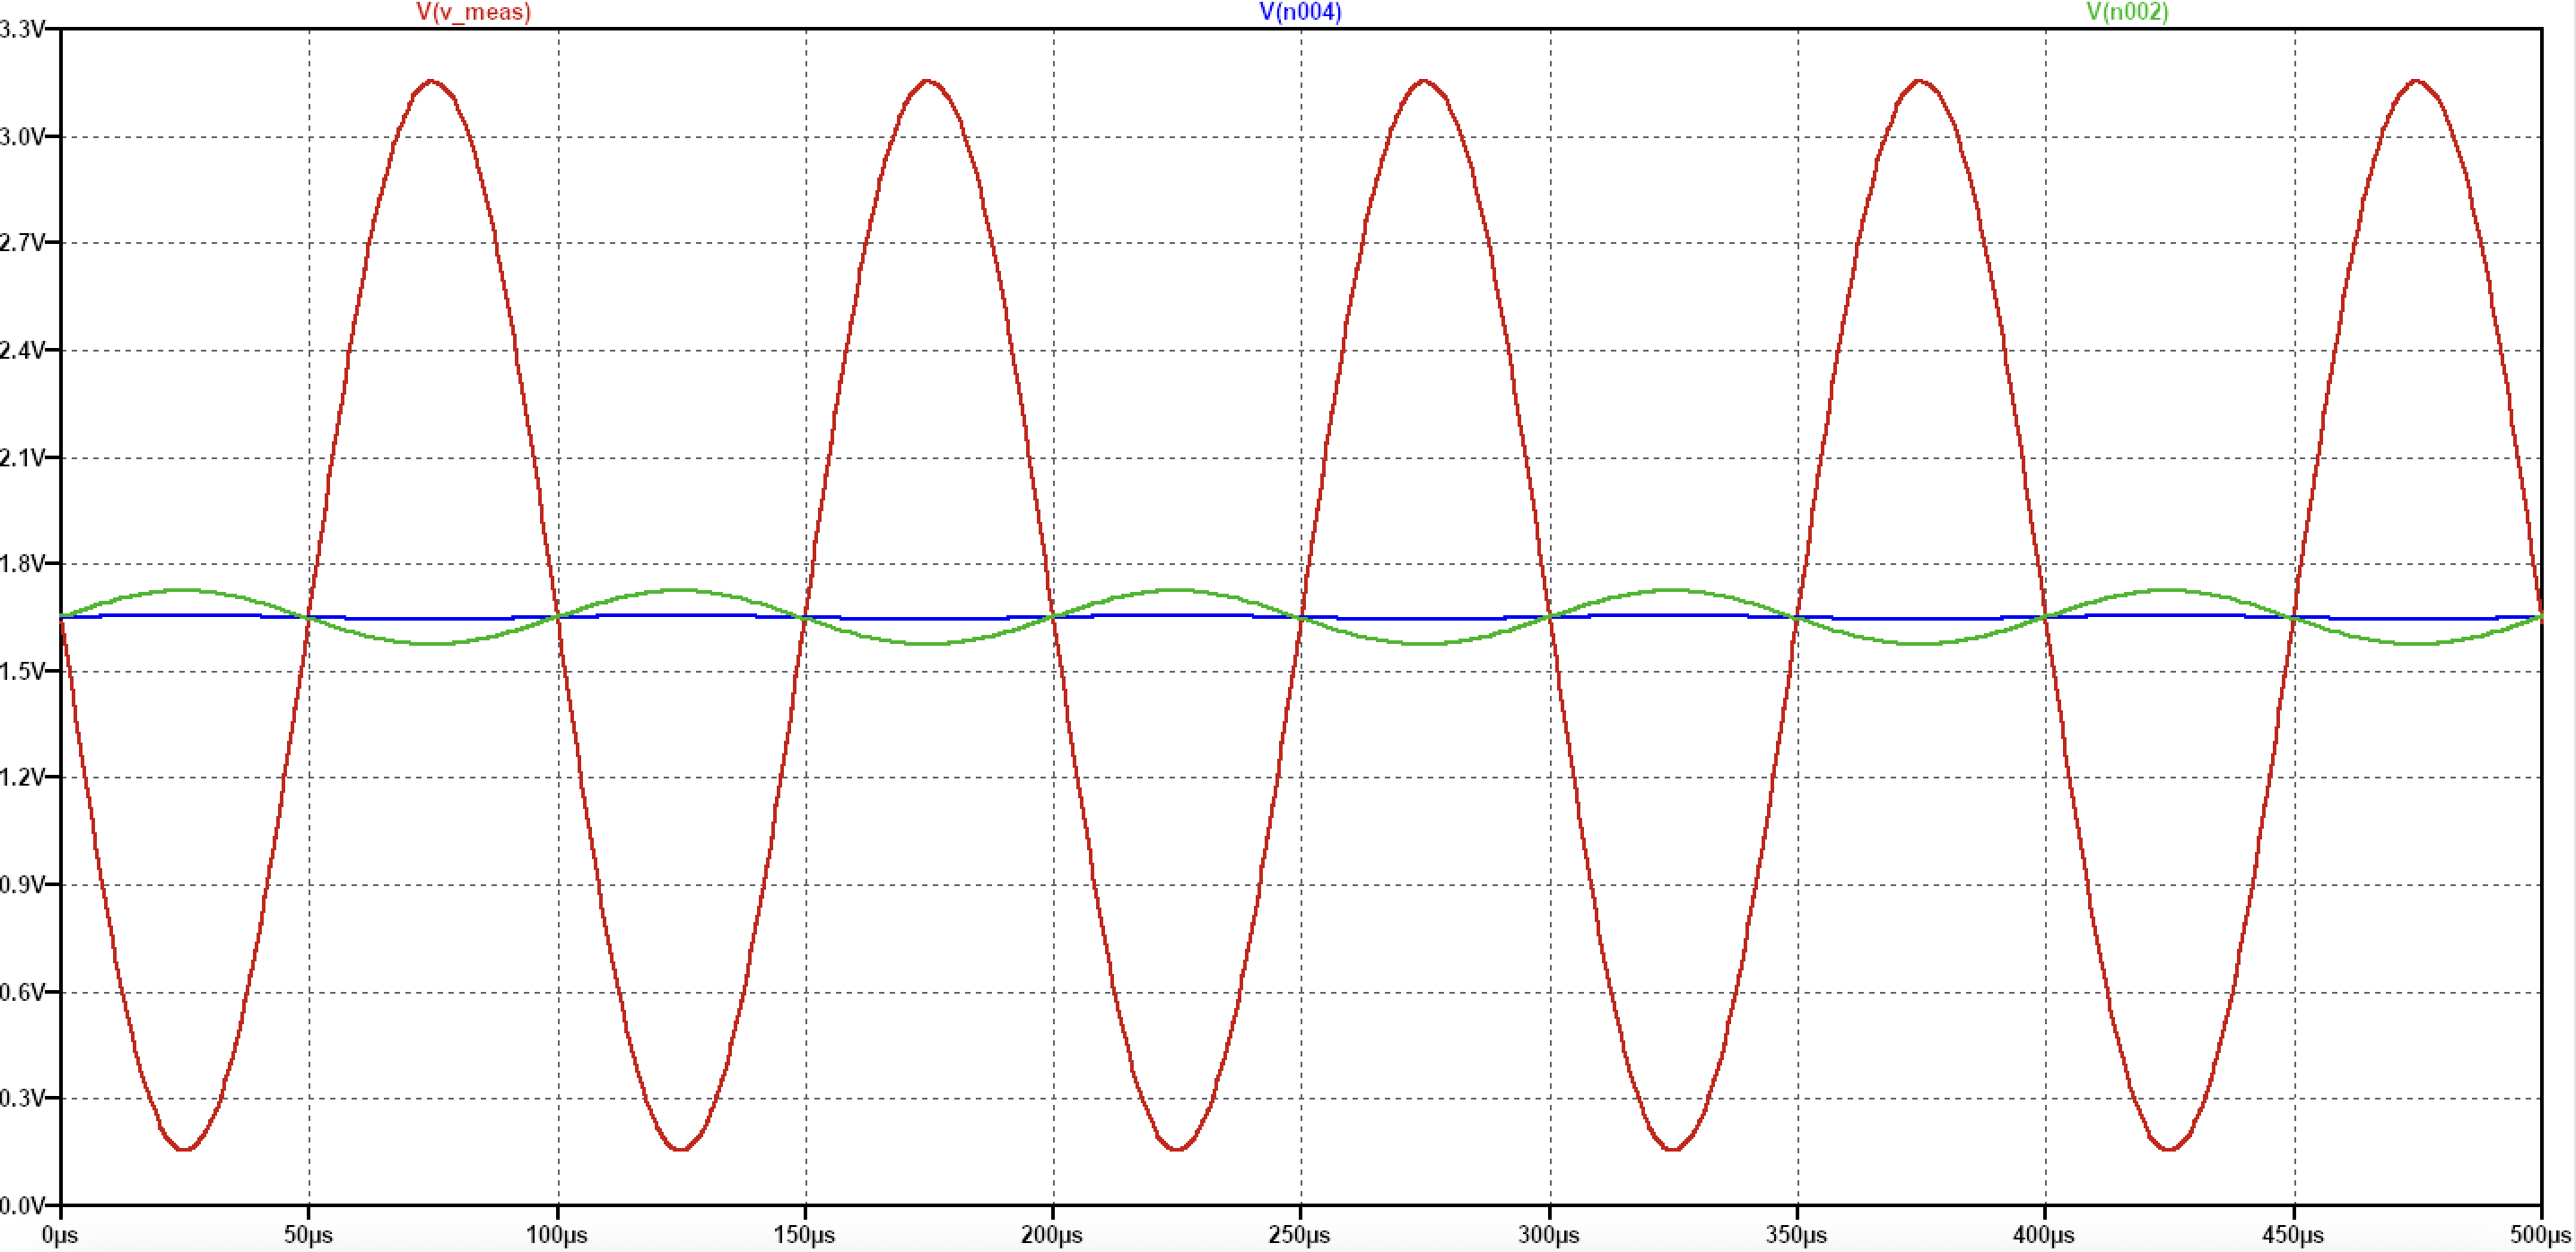
\includegraphics[width=\textwidth]{ExcitationStage.png}
        \caption{DAC output before and after AA-filter and attenuation}
        \label{fig:dac_filtering}
    \end{subfigure}\hfill
    \begin{subfigure}[b]{0.48\textwidth}
        \centering
        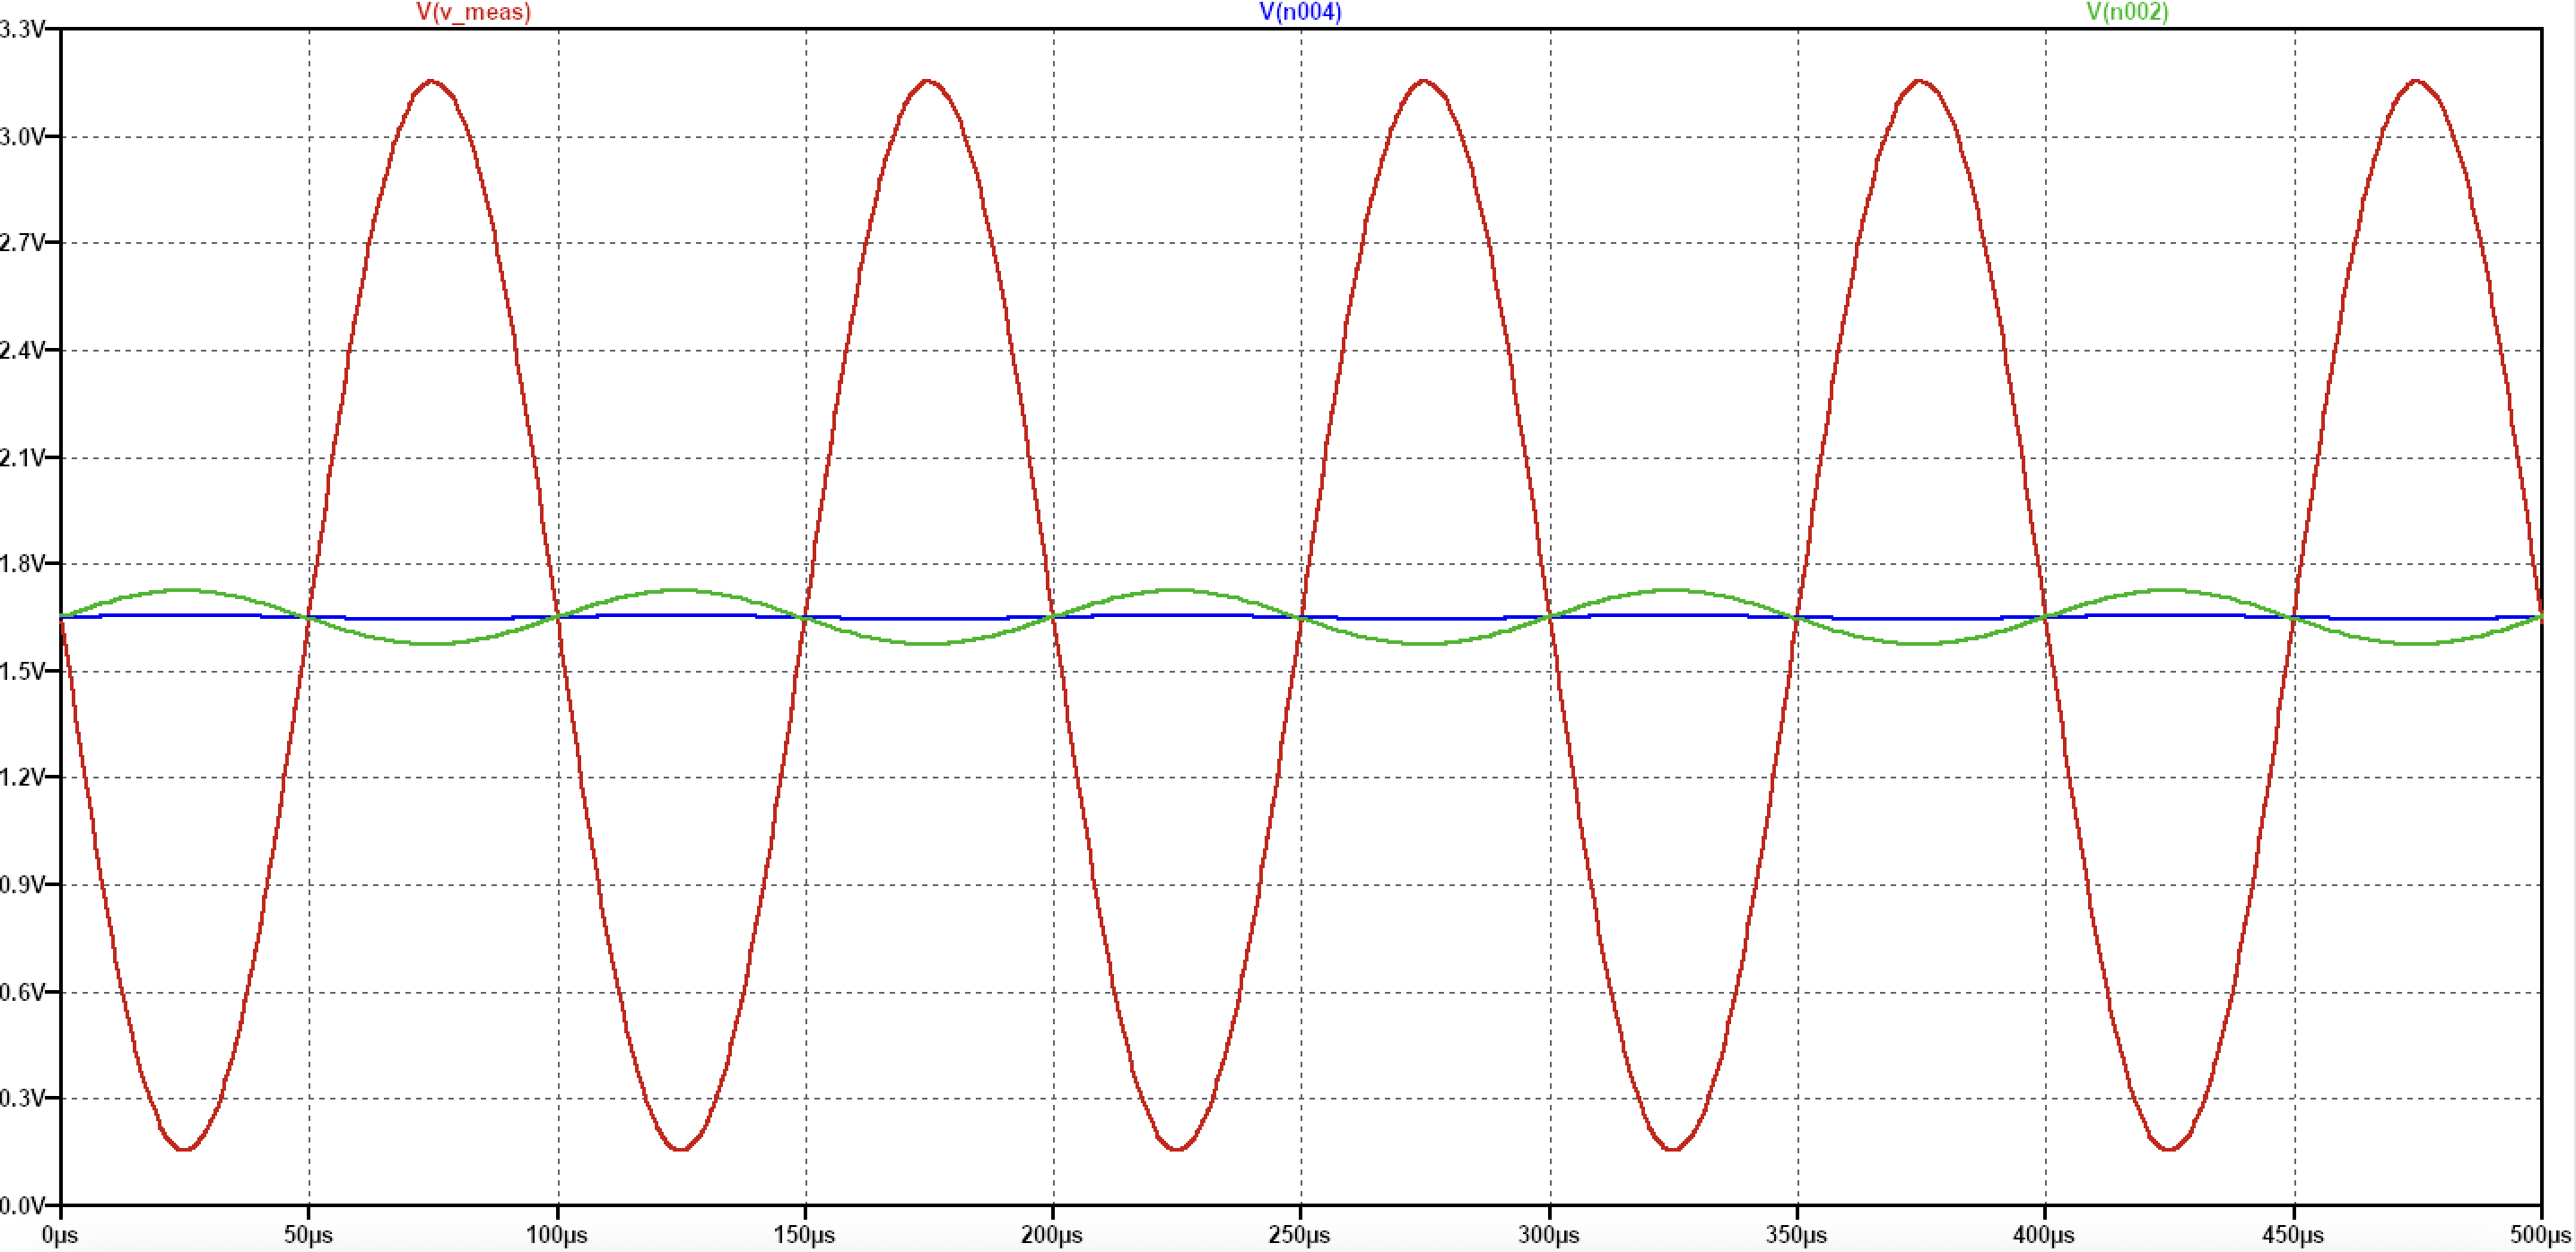
\includegraphics[width=\textwidth]{ExcitationStage.png}
        \caption{Current through simulated DUT}
        \label{fig:dut_current}
    \end{subfigure}
    \caption{Simulated excitation stage output and DUT response}
    \label{fig:excitation_sim}
\end{figure}

\subsection{Voltage measurement}
The voltage measurement stage was simulated with the INA331 and TLV9061 models to confirm the frequency response of the system. Figure \ref{fig:ina_freq} shows only a slight gain reduction of -0.02dB gain reduction at 100kHz and a -4.6\textdegree phase shift. Fig \ref{fig:v_meas_freq} shows the overall frequency response of the voltage measurement stage with the TLV9061 amplification stage contributing an additional -0.2dB gain reduction and -3.4\textdegree phase shift. This confirms that sufficient bandwidth is available for measurements up to 100kHz.

\begin{figure}[H]
    \centering
    \begin{minipage}{0.48\textwidth}
        \centering
        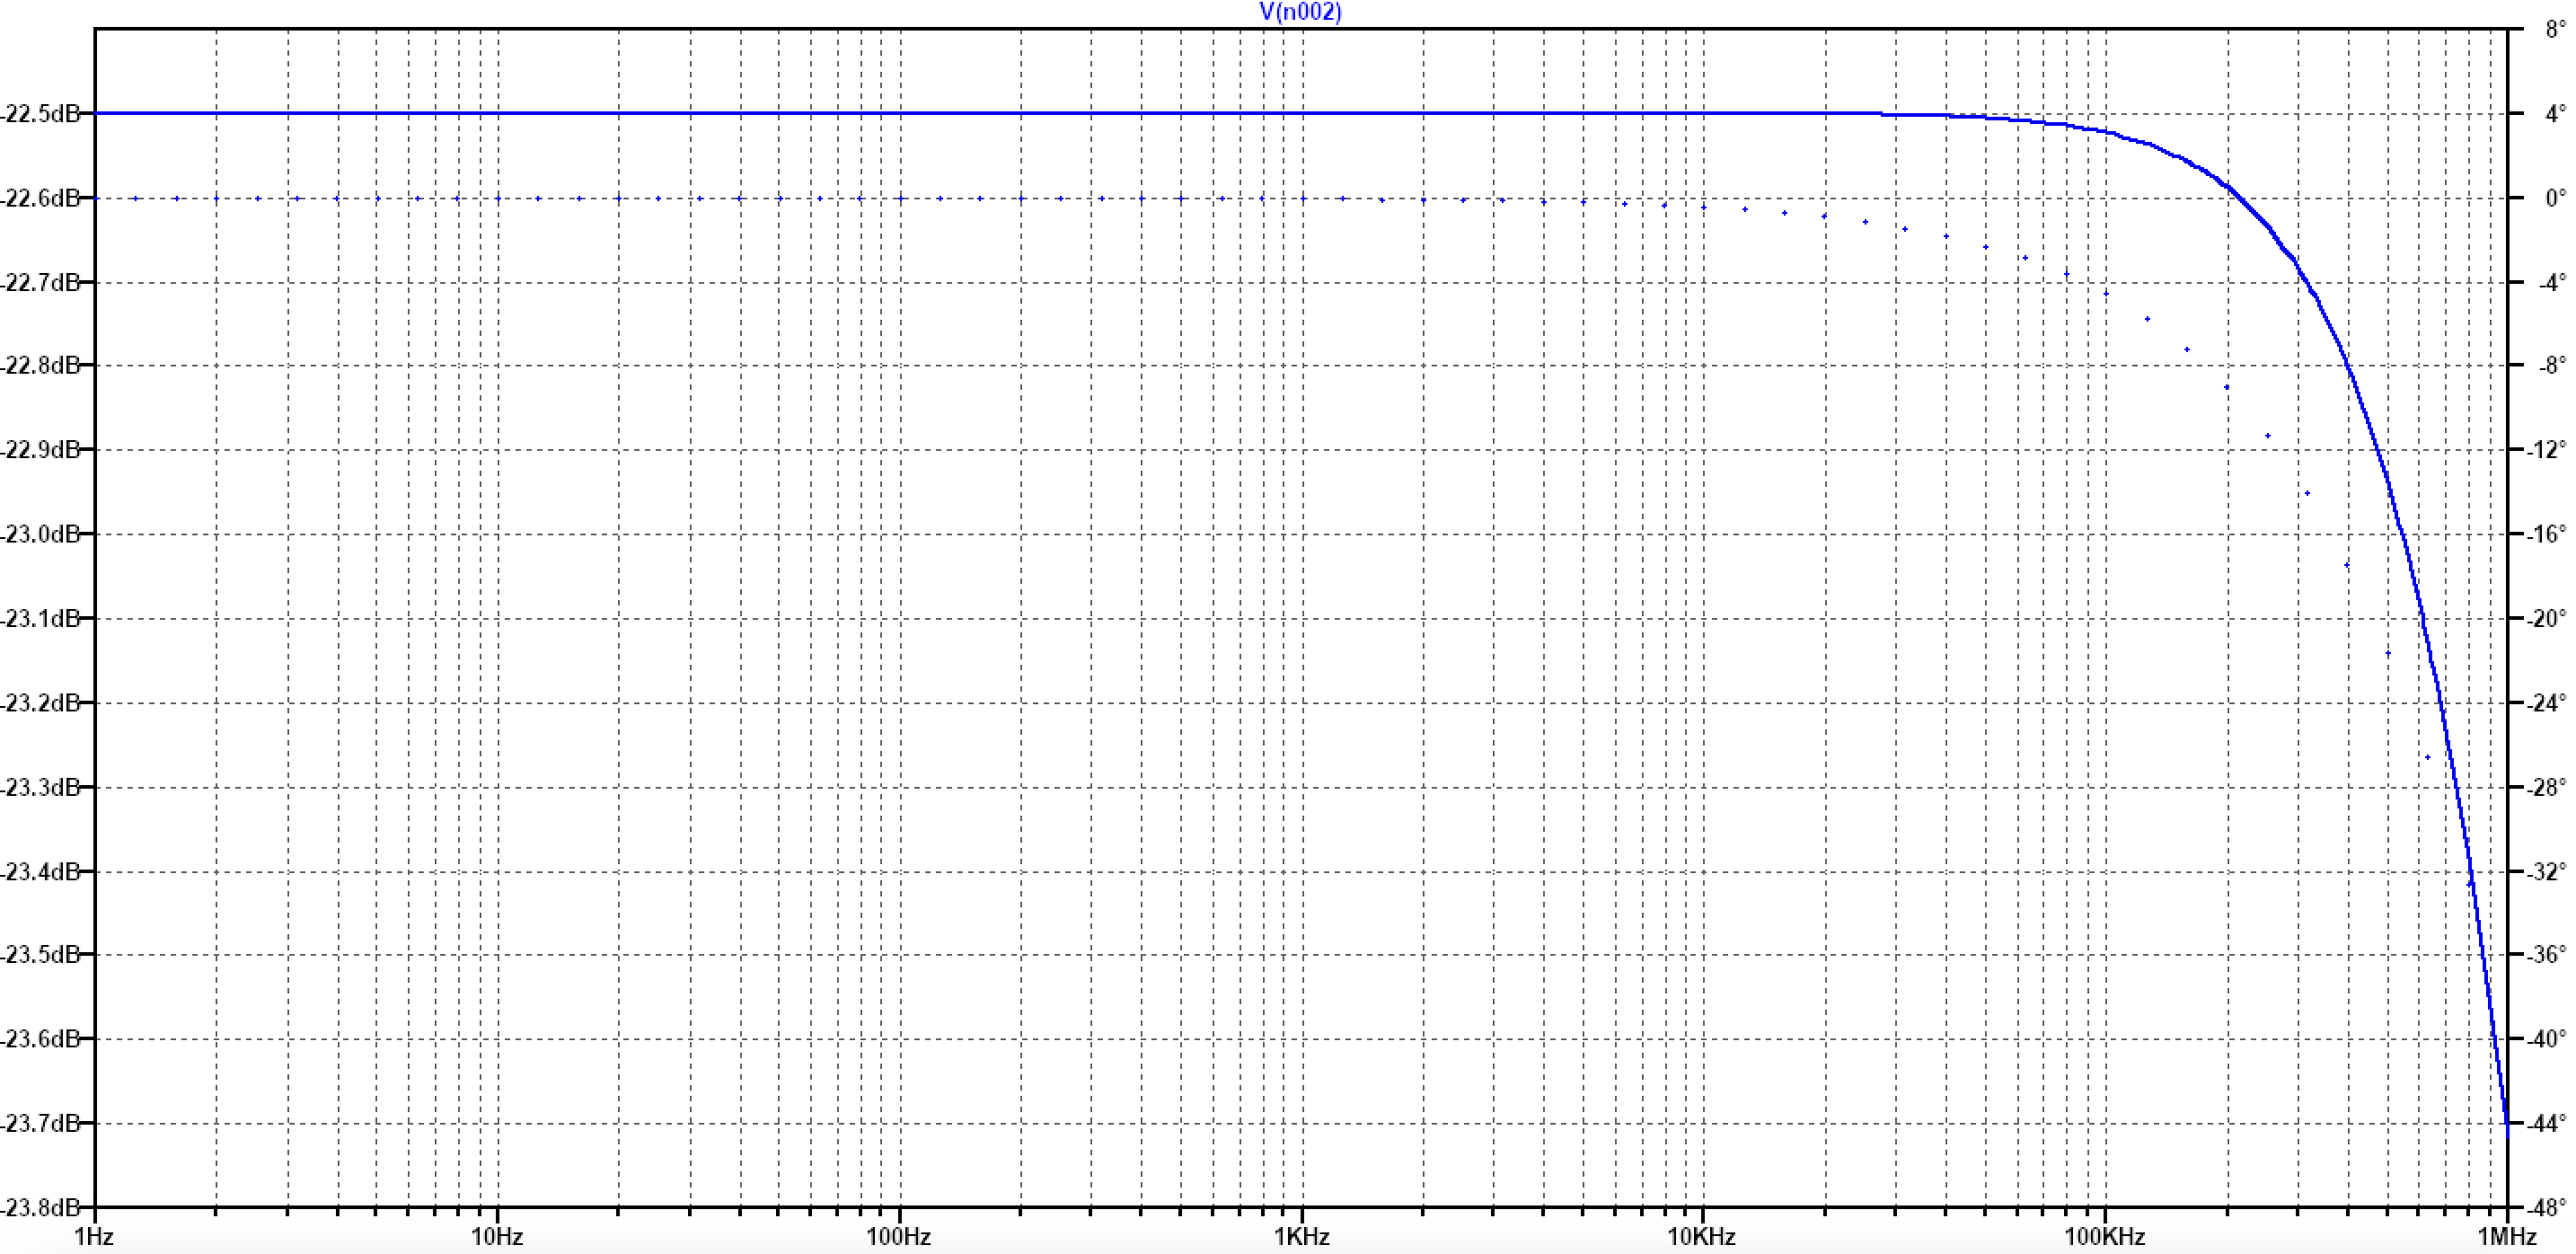
\includegraphics[width=\textwidth]{INA331FreqResponse.png}
        \caption{INA331 frequency response}
        \label{fig:ina_freq}
    \end{minipage}\hfill
    \begin{minipage}{0.48\textwidth}
        \centering
        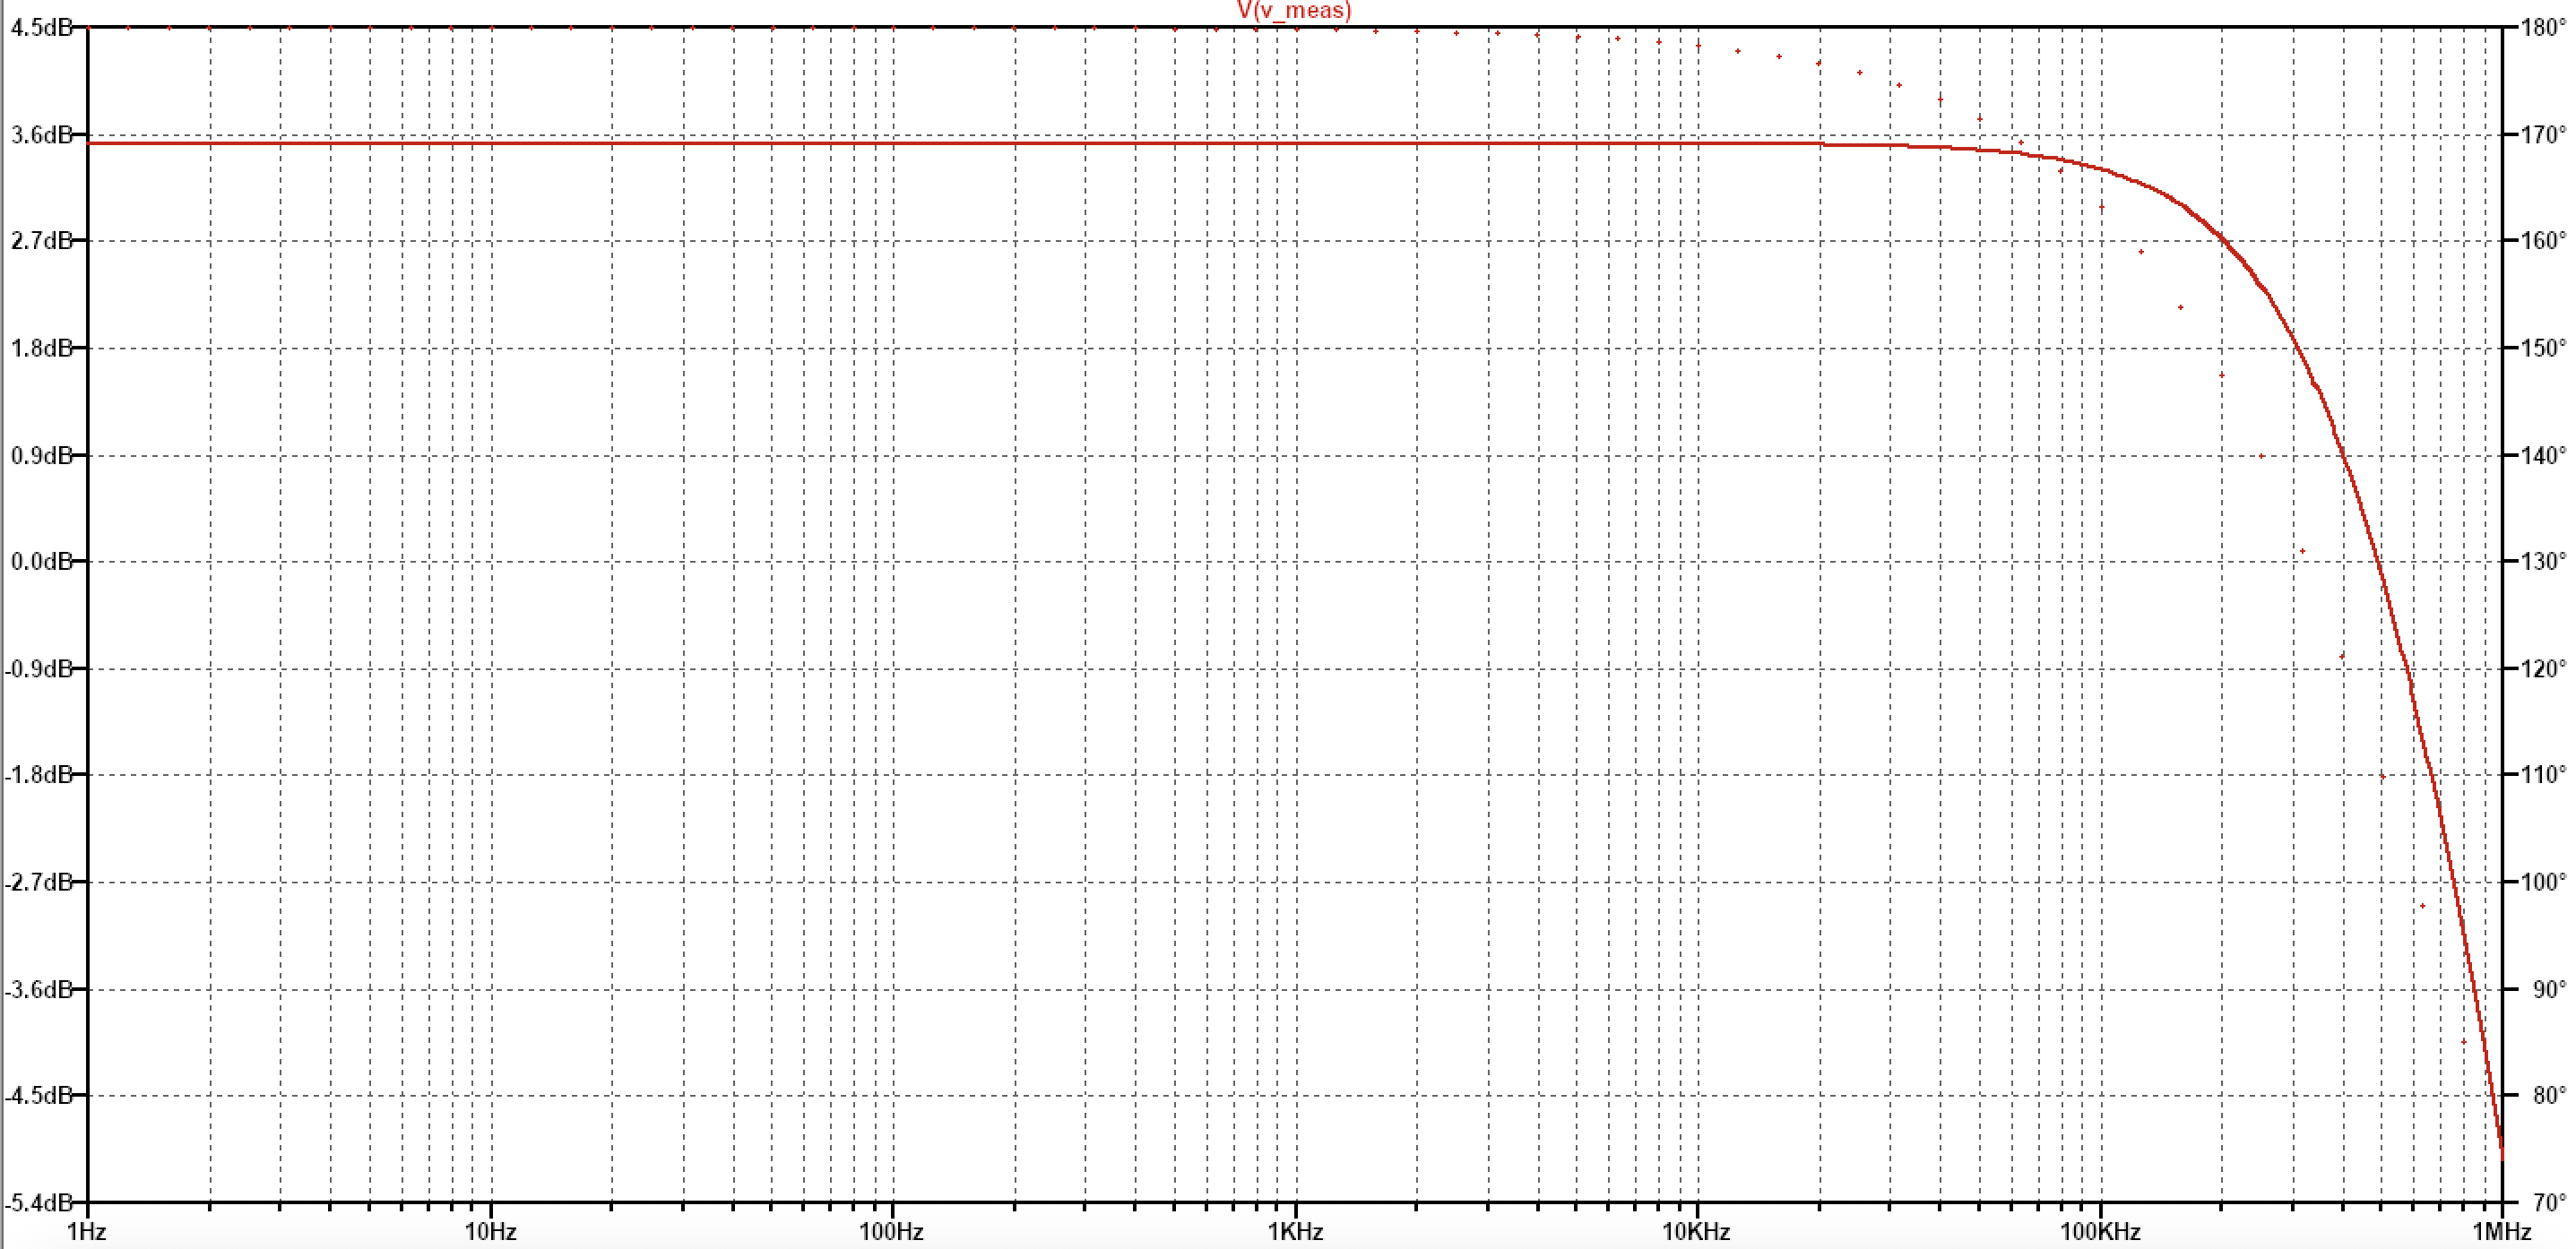
\includegraphics[width=\textwidth]{VmeasFreqResponse.png}
        \caption{Complete voltage measurement stage frequency response}
        \label{fig:v_meas_freq}
    \end{minipage}
\end{figure}

\subsection{Current measurement}
Due to problems porting the OPA3s328 PSpice model to LT Spice, the internal mux was not simulated. The PGA113 has no available PSpice model \cite{PGA113PspiceModel2022}, thus a standard inverting amplifier configuration using the TLV9061 was used to simulate the PGA stage. Figure \ref{fig:tia_freq} shows the frequency response of the TIA stage alone at both feedback resistor values. At 100 kHz with $R_F = 7.5~k\Omega$, the stage exhibits a gain increase of +0.136 dB and a phase shift of -15.4\textdegree. For $R_F = 37.5~\Omega$, the response shows a gain increase of +0.137 dB and a phase shift of -15.6\textdegree. The slight gain increase is due to very slight peaking in the frequency response before the eventual rolloff. This demonstrates a very flat frequency response well below the circuit's bandwidth limitations. Figure \ref{fig:i_meas_freq} shows the overall frequency response of the current measurement stage with the PGA and final amplification stages contributing an additional -0.25dB gain reduction and -4.8\textdegree phase shift. This confirms that sufficient bandwidth is available for measurements up to 100kHz.

To confirm the stability of the TIA circuit, Tian's method was used to plot the loop gain and phase margin for both the Radnles circuit using the \ac{CPE} and the simplified circuit using a constant capacitance as seen in figure \ref{fig:tia_stability} and Table \ref{tab:lt_tia_stability}. These results closely match the MatLab results in section \ref{subsec:design_cur}, confirming that the TIA design is stable without the need for feedback compensation.

\subsection{Complete System}
The individual subsystems were combined into a complete model including DAC and ADCs using sample-and-hold blocks. Transient analysis was done at a range of excitation frequencies. For frequency analysis the DAC and ADCs were excluded.

\section{PCB Design}\label{sec:PCB}
Beskryf filosofie en idees wat mee ingegaa het. Briefly discuss general PCB design principles wat design geguide het (Analogue ground plane etc). Beskryf beperkings van PCB manufactures wat inag geneem moes word (PCB size, layers, trace width via diamtre etc.). Noem briefly hoekom PCB in China eerder as Uni laat maak. Gaan deur design logic en discuss probleem met TIA. Include maybe final PCB diagram en langs dit foto van manufactured PCB.

All PCB design was done using KiCad due to its open-source nature and wide usage in industry. Due to the complexity of the circuit, JLC PCB was used for manufacturing rather than Stellenbosch University's in-house PCB manufacturing. \rephrase{There are substantial price differences between JLC's standard process and their more advanced processes (\textdollar 4 vs \textdollar 68)}. Table \ref{tab:jlc_limits} lists the key limits of JLC's standard PCB process that had to be taken into account. 

Another key consideration when designing the PCB was minimising noise and interference in the analogue circuitry. Given the limitations of a two-layer PCB, maintaining a continuous and low-impedance ground reference was a key priority, as a fully dedicated ground plane was not practical. To achieve this, both layers incorporated extensive ground copper pours connected through frequent stitching vias to minimise loop inductance and reduce \ac{EMI} coupling between layers. A single unified ground network was chosen over separate analogue and digital grounds, as is modern best practice for low-current mixed-signal systems \cite{WhatAreBasic}. Instead, the analogue and digital sections were physically partitioned, with sensitive analogue components and signal routed away from high-speed digital traces. Fencing vias were deployed along region boundaries to confine high-frequency digital currents and provide additional shielding for low-level analogue signals (Figure \ref{fig:via_fencing}).

Subsystems we're grouped together with jumpers connecting subsystems, allowing for easier debugging and testing. Care had to be taken in selecting the pin usage for both the STM32 and ESP32 as nearly all pins on both devices were used. The small package size of the OPA3S328 (24-pin DSBGA with 0.4 mm pitch) also posed challenges for routing. With a minimum pad diameter of 0.25 mm and 0.4 mm pitch, the clearance between pads is only 0.15 mm, meaning that traces could not be routed between pads. Usually this would be solved using via-in-pads, however, the minimum via hole diameter of 0.3 mm meant that this was not possible with JLC's low cost PCB manufacturing process. By only using 2 of the 3 internal switches, OUTSB3 could be used to route the common node of switch B to the non inverting input of the buffer op-amp (Figure \ref{fig:bga_routing}). This reduced the number of gain settings to 2 as mentioned in section \ref{subsec:design_cur}. 

The complete PCB schematic is shown in Appendix \ref{appendix:schematic} and the final PCB layout in Figure \ref{fig:final_pcb}.

\begin{table}[ht]
    \centering
    \caption{JLC PCB Standard Manufacturing Process Limits}
    \label{tab:jlc_limits}
    \begin{tabular}{ll}
        \hline
        \textbf{Parameter} & \textbf{Limit} \\
        \hline
        Minimum Trace Width & \SI{0.1}{\milli\meter} (4 mil) \\
        Minimum Trace Spacing & \SI{0.1}{\milli\meter} (4 mil) \\
        Minimum Via Diameter & \SI{0.45}{\milli\meter} \\
        Minimum Via Hole Diameter & \SI{0.3}{\milli\meter} \\
        Minimum BGA Pad Diameter & \SI{0.25}{\milli\meter} \\
        Maximum Board Size & \SI{100}{\milli\meter} × \SI{100}{\milli\meter} \\
        Number of Layers & 2, 4, or 6 layers \\
        \hline
    \end{tabular}
\end{table}

\begin{figure}[ht]
    \centering
    \begin{subfigure}[b]{0.48\textwidth}
        \centering
        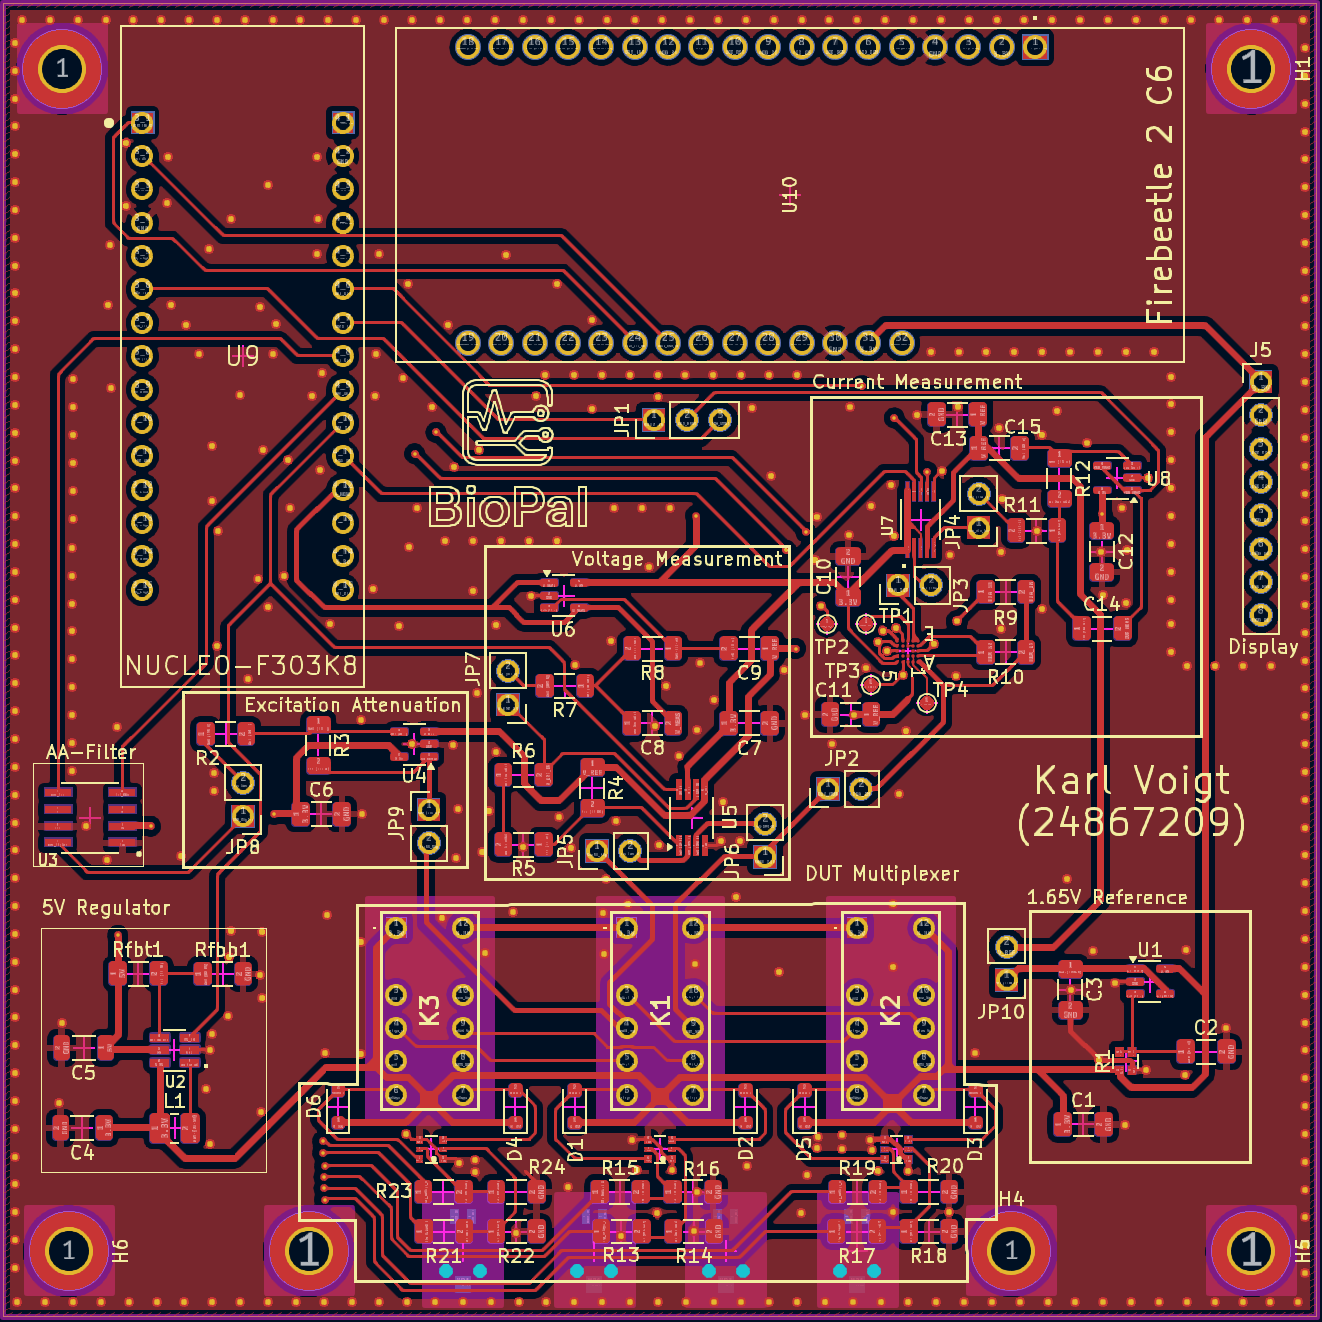
\includegraphics[width=\textwidth]{BioPal_Front.png}
        \caption{PCB front layout}
        \label{fig:pcb_front}
    \end{subfigure}\hfill
    \begin{subfigure}[b]{0.48\textwidth}
        \centering
        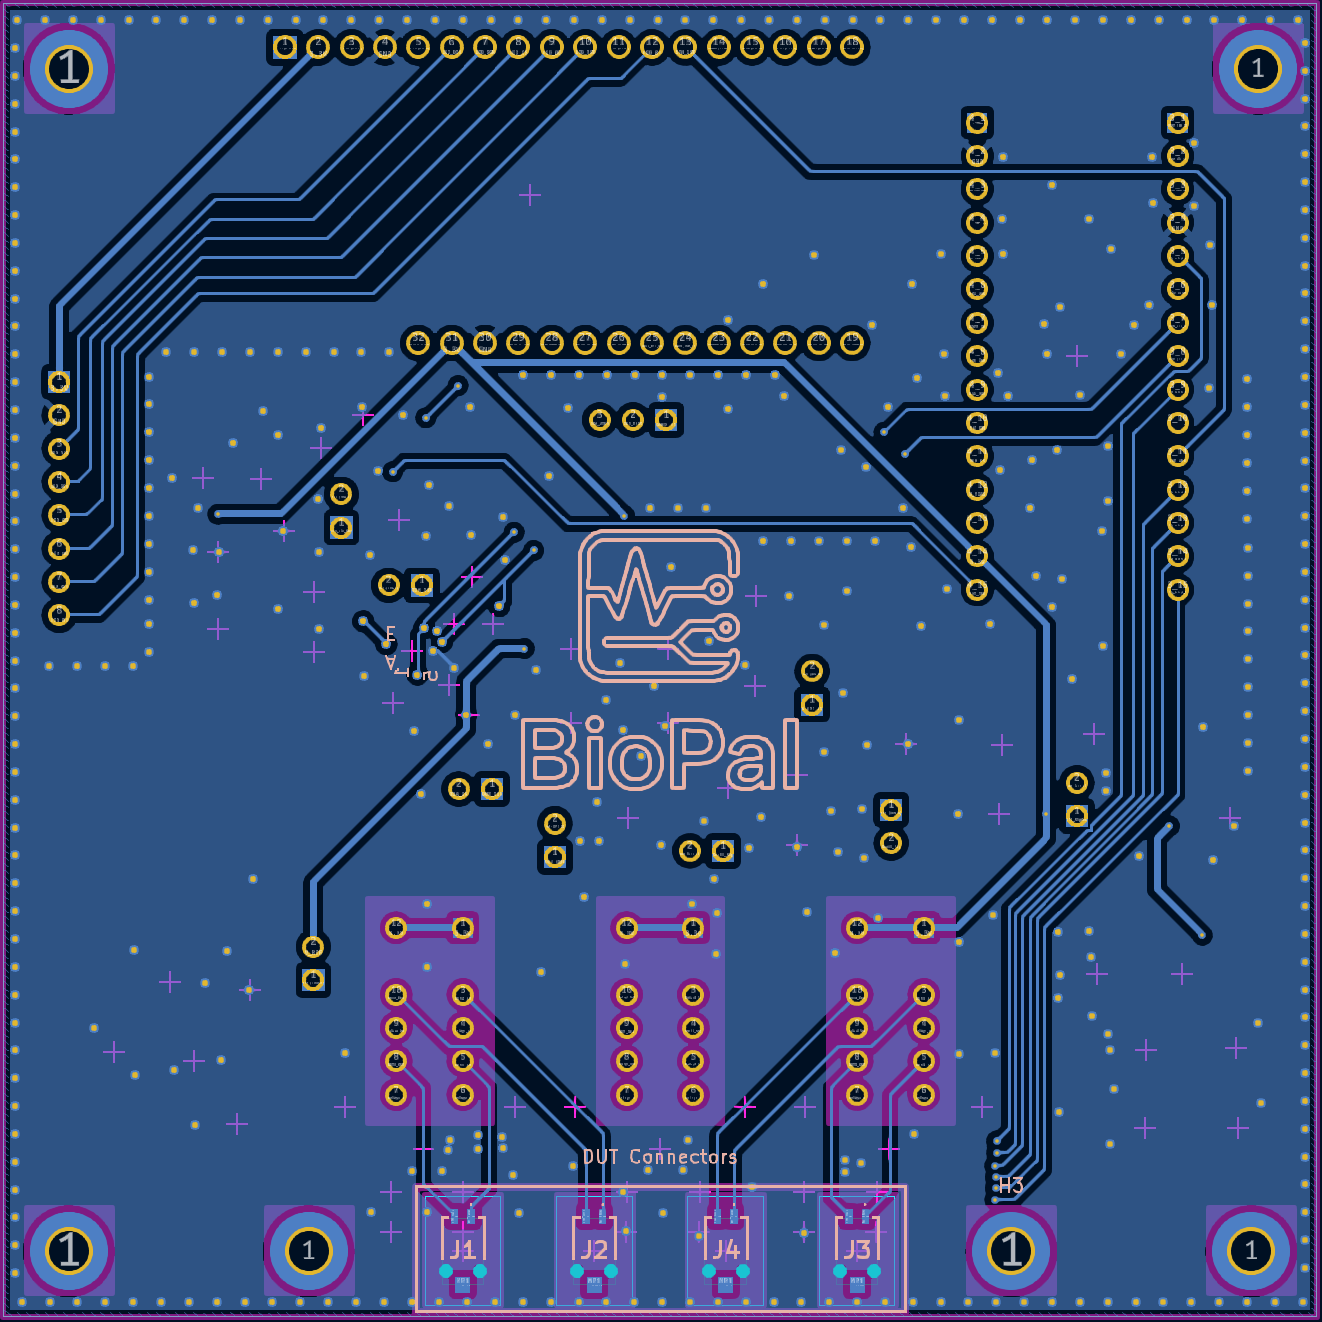
\includegraphics[width=\textwidth]{BioPal_Back.png}
        \caption{PCB back layout}
        \label{fig:pcb_back}
    \end{subfigure}
    \caption{Final PCB layout}
    \label{fig:pcb_layout}
\end{figure}

\begin{figure}[ht]
    \centering
    \begin{minipage}{0.4\textwidth}
        \centering
        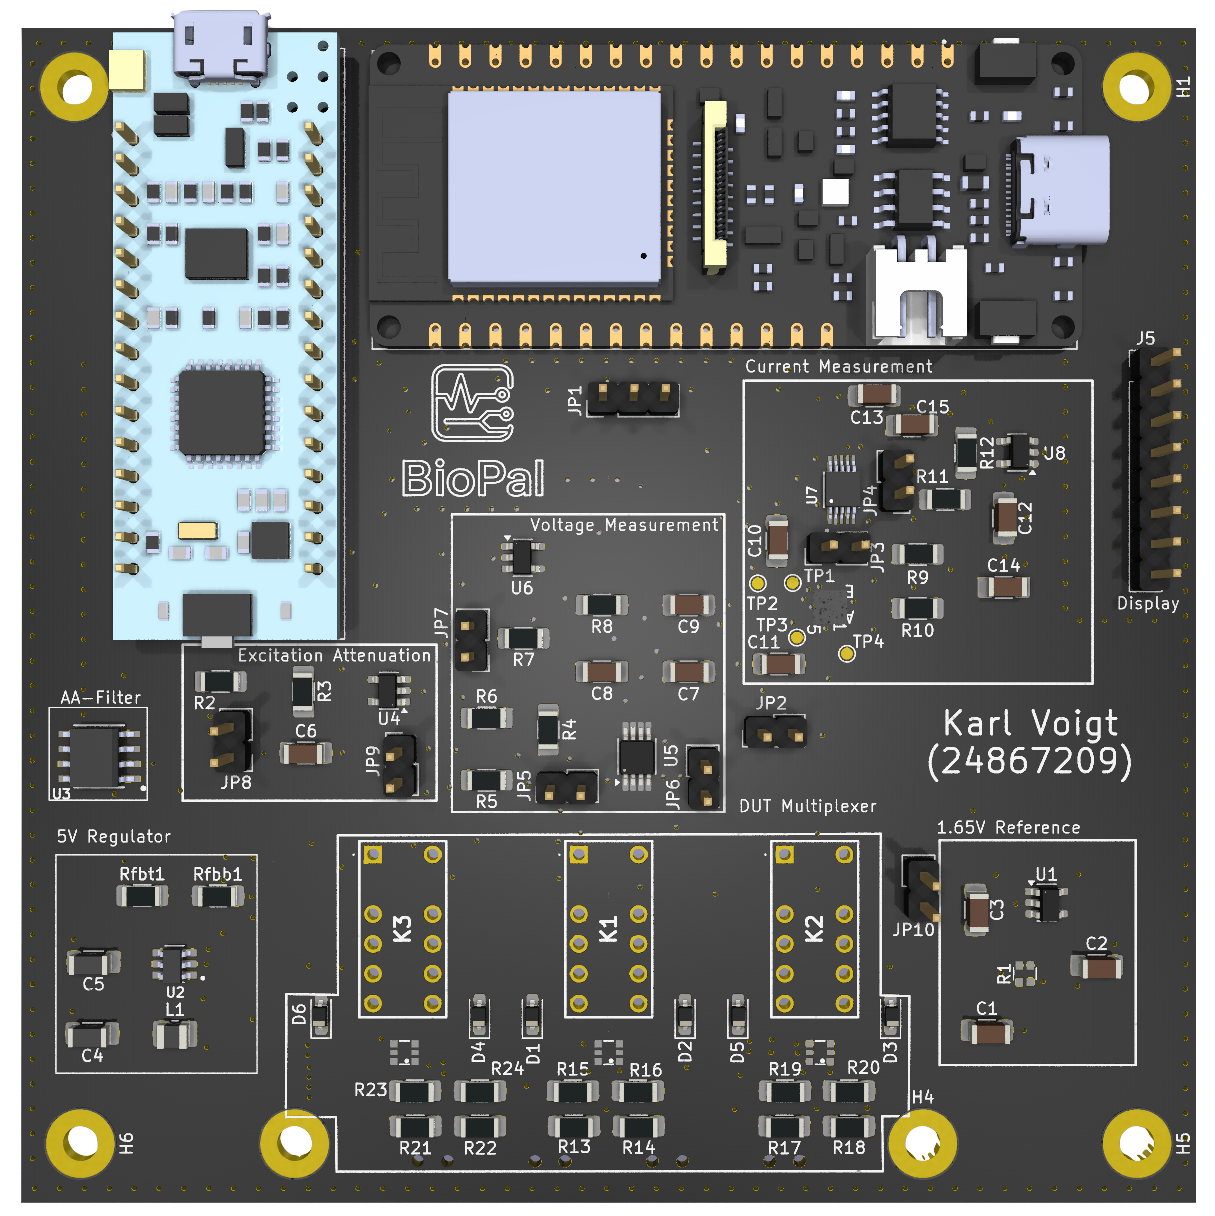
\includegraphics[width=\textwidth]{BioPal_render.png}
        \caption{Final PCB render}
        \label{fig:final_pcb}
    \end{minipage}\hfill
    \begin{minipage}{0.35\textwidth}
        \centering
        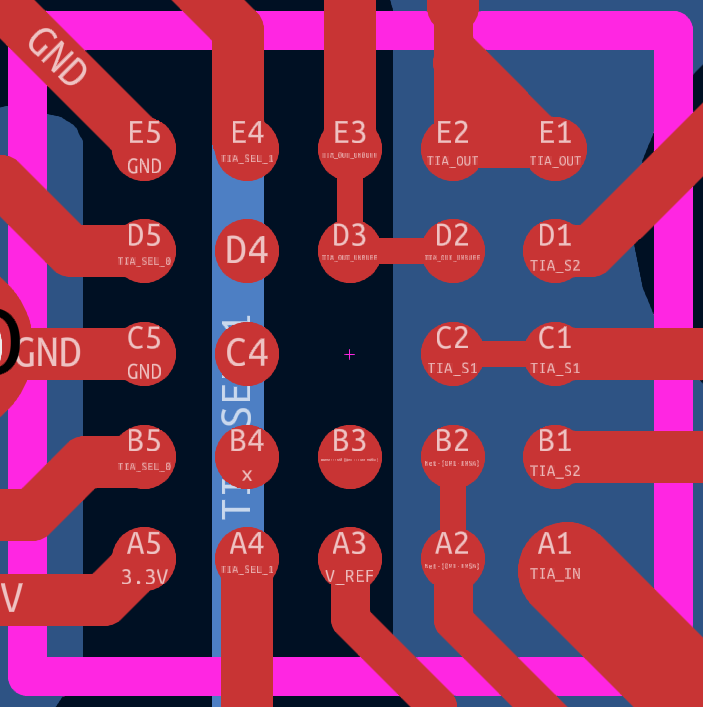
\includegraphics[width=\textwidth]{BGA_Routing.png}
        \caption{\\OPA3S328 BGA routing solution}
        \label{fig:bga_routing}
    \end{minipage}
\end{figure}

\section{Firmware Development}
Inculde flow diagram.

\subsection{ESP}
Vertel van wat ons wil bereik en hoekom. Discuss libraries used. Discuss maybe issues rondom C6 en hoe dit gesolve is en hoekom die C6 steeds die rgete keuse was.

\subsection{STM}
Probleme met arm library te groot. Discuss met flow chart hoe DMA en als met DAC en ADC interact en dan UART en badies program flow. Delve into limits van STM en maybe briefly setup van DAC en ADC.

\label{chap:design}